% ============================================================
%  日本語版 — Every edge-perimeter-minimizing polyhex ...
%  Compile with:  xelatex main_ja.tex ; bibtex main_ja ; xelatex ×2
%  英語版 rev3（2026-09-28 review corrections）に同期した日本語版。
%  ラベル名は英語版と同一に保ってある。
% ============================================================
\documentclass[11pt]{article}
\usepackage{amsmath,amssymb,amsthm}
\usepackage[margin=1in]{geometry}
\usepackage{array}
\usepackage{tabularx}
\usepackage{booktabs}
\usepackage{tikz}
\usepackage{float}
\usepackage{fontspec}
\setmainfont{Noto Serif CJK JP}
\newfontfamily\jasf{Noto Sans CJK JP}
\XeTeXlinebreaklocale "ja"
\XeTeXlinebreakskip = 0pt plus 1pt minus 0.1pt
\usepackage[hidelinks]{hyperref}

\theoremstyle{plain}
\newtheorem{theorem}{定理}[section]
\newtheorem{lemma}[theorem]{補題}
\newtheorem{proposition}[theorem]{命題}
\newtheorem{corollary}[theorem]{系}
\theoremstyle{definition}
\newtheorem{definition}[theorem]{定義}
\newtheorem{example}[theorem]{例}
\newtheorem{fact}[theorem]{事実}
\newtheorem{observation}[theorem]{観察}
\theoremstyle{remark}
\newtheorem{remark}[theorem]{注意}
\renewcommand{\proofname}{証明}
\renewcommand{\figurename}{図}
\renewcommand{\tablename}{表}
\renewcommand{\refname}{参考文献}
\renewcommand{\abstractname}{概要}
\renewcommand{\contentsname}{目次}

\newcommand{\Z}{\mathbb{Z}}
\newcommand{\sm}{\setminus}
\DeclareMathOperator{\exc}{exc}
\newcommand{\dg}{\operatorname{deg}}

\title{辺周長最小 polyhex の最短辺 skeleton}
\author{宇都宮 英之}
\date{}

\begin{document}
\maketitle

\begin{abstract}
polyhex とは六角タイリングのセルからなる有限連結集合であり，その辺周長とは，polyhex を
その補集合から隔てる単位辺の本数である．セル数を与えたときの最小辺周長は古典的に知られて
おり，各サイズに一つずつ最小配置を並べた入れ子列が一本存在することも同様である．本稿は，
\emph{すべての}最小配置に関する構造的な主張を証明する．3 セル以上の最小配置から任意の最短
extreme line を削除すると，そのセル数に対する最小辺半周長（\emph{閾値}）がちょうど一段下がった
最小配置が残り，削除した線は，辺周長
がそのサイズにおける最小値を高々 2 だけ上回る配置を経由して一セルずつ戻せる．したがって
任意の最小配置は，そのような削除で結ばれた最小配置の鎖の上にあり，任意の最小配置は一セル
から出発して隣接する一セルずつを加えることで，辺周長超過が常に 2 以下のまま構築できる．
定数 2 は下げられない．最小配置の骨格はすべての最小配置について存在するが，単一セルの
水準では，すべての最小配置が最小配置の入れ子列の上にあるわけではない．証明は配置の tight
hull，その厳密な defect 恒等式，および閾値が 6 を法として 3 または 5 である plateau の開始点
における剛性に基づく．
\end{abstract}

\noindent\textit{2020 Mathematics Subject Classification.} Primary 05B50; Secondary 05C35,
52C20.

\noindent\textit{Key words and phrases.} polyhex, edge-isoperimetric problem, minimum edge
perimeter, edge-perimeter minimizer, nested solutions, one-cell growth sequence, triangular
lattice, hexagonal tiling.

\section{序論}\label{sec:intro}

\subsection{問題}\label{sec:0.1}

対象は六角タイリングのセルである．\emph{polyhex} とはセルの有限連結集合であり，その
\emph{辺周長} \(p(S)\) とは，ちょうど一方の側だけが \(S\) に属する単位辺の本数である．
\(N\) セルの polyhex が取りうる最小の辺周長を \(p_{\min}(N)\) と書き，
\[
   \exc(S):=p(S)-p_{\min}(|S|)
\]
を\emph{超過}と呼ぶ．\(\exc=0\) である polyhex を\emph{最小配置}と呼ぶ．

静的な問題，すなわち \(p_{\min}(N)\) は何か，最小配置はどのような形をしているか，は古典的で
ある．本稿の問いは動的である．最小配置は完成した対象であるが，それを\emph{組み立てる}ことは
できるか．一セルずつ加えながら，最適性の近傍から一度も離れずに組み立てられるか．形式的に
述べれば，\(N\) セルの最小配置 \(S\) が与えられたとき，
\[
   S_{1}\subset S_{2}\subset\cdots\subset S_{N}=S,\qquad |S_{k}|=k,
\]
なる polyhex の鎖であって，各段階が隣接する一セルの追加であり，どの \(S_{k}\) も超過が小さい
ものは存在するか，という問いである．

困難の所在は二点にある．第一に，全段階で \(\exc(S_{k})=0\) を要求することはできない．本稿は
13 セルの最小配置であって，どの一セルを取り除いても 12 セルの最小配置が残らないものを与える．
第二に，この問いを素朴に貪欲に読むと偽になる．超過が高々 2 の配置であれば，超過を高々 2 に
保つ一セル削除が必ずあるとは限らず，注意~\ref{rem:x31} の 31 セルの方向凸な例にはそのような
下降の手がない．したがってクラス \(\{\exc\le2\}\) 全体を，常に使える一手を持つ一セル降下
帰納法の状態空間にすることはできない．

\subsection{結果}\label{sec:0.2}

答えは，成長が最小配置からなる\emph{骨格}を持つ，ということである．polyhex \(S\) について，
六本の \emph{extreme line} とは三つの格子方向それぞれにおける最外の占有線であり，
\emph{最短} extreme line とは \(S\) のセルを最も少なく持つものをいう．最小配置では各
extreme line 上の \(S\) のセルは連続する run をなすが，これは定理~\ref{thm:capacity}(d)
で証明される事実であり，定義~\ref{def:traces} はその性質を持つ polyhex のクラス上で
support trace を定める．
\(g(N):=\lceil\sqrt{12N-3}\,\rceil\) とおけば，第~\ref{sec:capacity}~節で再掲する古典的結果により
\(p_{\min}(N)=2g(N)\) である．本稿では \(g(N)\) を \(N\) の\emph{閾値}と呼ぶ．これは
\(N\) セル polyhex が持ちうる最小の辺半周長であり，連続する複数の \(N\) にわたって一定に
なる区間を \emph{plateau} と呼ぶ．polyhex \(S\) の\emph{超過}は
\[
  \exc(S)=p(S)-p_{\min}(|S|)=2\bigl(\sigma(S)-g(|S|)\bigr),
\]
ここで \(\sigma(S)=p(S)/2\) は辺半周長である．

\begin{theorem}[最短辺 skeleton]\label{thm:intro-skel}
\(S\) を \(|S|\ge3\) の辺周長最小配置，\(\Lambda\) を \(S\) の任意の最短 extreme line とする．
このとき \(S\sm\Lambda\) は \(g(|S\sm\Lambda|)=g(|S|)-1\) なる辺周長最小配置であり，
\(S\cap\Lambda\) のセルは超過が高々 2 の polyhex を経由して一つずつ戻すことができる．
\end{theorem}

これを反復すると，任意の最小配置 \(S\) は最小配置の鎖
\(S=T_{0}\supset T_{1}\supset\cdots\supset T_{k}\)，\(|T_{k}|\le2\) であって各々が直前のもの
から最短 extreme line を削除して得られるものを持つ．各段を補間して逆向きに読めば成長の主張
になる．

\begin{theorem}[一セル成長]\label{thm:intro-main}
\(S\) を辺周長最小の \(N\) セル polyhex とする．このとき polyhex の列
\(S_{1}\subset\cdots\subset S_{N}=S\)，\(|S_{k}|=k\)，であって次を満たすものが存在する．
\begin{enumerate}
\item[(a)] 各 \(k<N\) について，\(S_{k+1}\) は \(S_{k}\) に隣接する一セルを加えて得られる．
\item[(b)] 各 \(k\) について \(\exc(S_{k})\le2\)．
\end{enumerate}
\end{theorem}

\(N\) セルの最小配置全体を \(\mathcal{M}_{N}\)，一セルから出発し超過が 2 を超えない一セル成長
で到達できる \(N\) セル polyhex 全体を \(\mathcal{R}_{N}\) と書けば
\(\mathcal{M}_{N}\subseteq\mathcal{R}_{N}\)．候補生成をこの種の成長に制限しても最小配置を
一つも取りこぼさない．

\begin{theorem}[定数の最適性]\label{thm:intro-sharp}
定理~\ref{thm:intro-main} の定数 2 を下げることはできない．
\end{theorem}

\(p\) と \(p_{\min}\) はいずれも偶数なので超過は常に非負の偶整数であり，2 より小さい一様な
上界は実質的に 0 しかない．上で触れた 13 セルの配置がそれを排除する．
定理~\ref{thm:intro-skel} と~\ref{thm:intro-sharp} を合わせると代価の所在が正確に定まる．
最小配置の骨格は常に最適に保てるが，超過 2 が消費されるのは一本の extreme line をセルごとに
組み直している間だけである．

\subsection{証明の仕組み}\label{sec:0.3}

三つの材料が議論を支える．第一に，すべての最小配置は\emph{方向凸}である．すなわち三つの格子
方向のそれぞれに沿って，各線上のトレースが単一の run である．これは配置の \emph{tight hull}，
すなわち extreme line が張る格子六角形との比較から従う．その hull のセル数は六つの辺長による
厳密な \emph{defect 恒等式}を満たす．同じ恒等式が容量関数
\(M(t)=\lfloor(t^{2}+3)/12\rfloor\)——辺半周長の予算 \(t\) の中に収まる最大セル数——を与え，
それとともに \(p_{\min}\) の公式を与える．

第二に，hull の六つの辺長の和は占有線数よりちょうど 3 だけ大きいので，閾値 \(\sigma\) の
最小配置の最短 extreme line は高々 \(\lfloor(\sigma+3)/6\rfloor\) セルしか持たない．6 を法とする
剰余の計算により，その数だけのセルを最小配置から削除すると閾値が一段下の最小配置に着地する
ことが分かる．ただし，閾値が 6 を法として 3 または 5 であり，最小配置がその plateau のまさに
先頭にあり，最短線が上界いっぱいの長さである場合だけは例外となりうる．

第三に，その例外的な状況で最短トレースが上界に達したと仮定すれば，hull は正六角形か，一組の
対辺を 1 だけ延ばした正六角形に強制され，その境界は最小配置が hull を完全に埋めることを強制
する．しかし plateau の先頭はその六角形より真に少ないセル数しか持たない．この\emph{剛性}が
最後の場合を閉じる．削除した線を一セルずつ戻す間，周長は出発時の値を超えない一方，閾値は
既に一段下がっている．超過 2 はここから来る．

\subsection{計算の役割}\label{sec:0.4}

本稿のどの定理も有限の数え上げに依存しない．定理~\ref{thm:intro-sharp} も同様である．計算は
第~\ref{sec:computation}~節において二つの目的にのみ用いる．最小配置が最小配置のみを経由する
成長鎖を持たなくなる最小のサイズが 13 であることを，完全な数え上げによって決定するため——
これは解析的な議論が答えない問いである——と，本稿の主張を独立な実装で小さなサイズにおいて
再検査するためである．

\subsection{先行研究との関係}\label{sec:0.5}

公式 \(p_{\min}(N)=2\lceil\sqrt{12N-3}\rceil\) は Harary と Harborth
\cite{HararyHarborth1976} によるもので，三つのユークリッド的タイリングにおける extremal
animal を決定したものである．これは \(b\) をセル間の隣接対の個数として
\(p=6N-2b\) と置けば，平面上の互いに内部が重ならない \(N\) 個の合同円板について接触対の
最大数を \(\lfloor3N-\sqrt{12N-3}\rfloor\) とする Harborth の先行公式
\cite{Harborth1974} に対応する．本稿は第~\ref{sec:capacity}~節で自足的な導出を与える．証明が
必要とするのは値そのものではなく，値を生み出す hull の機構だからである．

その機構自体は既知の領域に近く，どこが既知であるかは明示しておく．容量関数 \(M(t)\) は，
代入 \(p=t+3\) の下で，Fülep と Sieben が \emph{site} 周長について決定した最大サイズ関数
\cite[Proposition~5.10]{FulepSieben2010} と一致する．また本稿の hull defect 恒等式は，彼らの
polyiamond の恒等式 \cite[Lemma~3.3]{FulepSieben2010} を，同論文第 5 節の三角格子と六角格子の
双対を通して移したものである．唯一の例外値までが両側で一致する．第~\ref{sec:hulls}~節が
加えているのはこれらの恒等式ではなく，辺周長変数による定式化であり，本稿の残りが消費するのは
その形である．

Barequet と Ben-Shachar \cite{BarequetBenShachar2022} は最小 \emph{site} 周長 animal を
研究し，inflation——animal にその周長層全体を加える操作——があるサイズの最小配置とより大きい
サイズの最小配置との間に全単射を誘導することを示して，ベンゼノイド炭化水素の化学で観察されて
いた constant-isomer 現象を証明した．続く論文 \cite{BarequetBenShachar2023} は最小 site 周長
animal を数え上げるアルゴリズムを与える．この系譜は本稿と三点で異なる．汎関数が辺周長では
なく site 周長であること，inflation が配置全体に作用してサイズを一セルではなく周長の分だけ
進めること，そして最適性の要求が関係づける二つのサイズにのみ課され，途中の各サイズには課さ
れないことである．本稿は二つの周長の概念をどこでも同一視せず，一方に関する結果を他方へ移さ
ない．

\emph{すべての}最小配置を扱う先行研究として最も近いのは Davoli, Piovano, Stefanelli
\cite{DavoliPiovanoStefanelli2017} である．彼らは三角格子上の辺等周問題——下で述べる同一視に
より本稿と同じ問題——を扱い，すべての最小配置の特徴づけを目的としている．同論文の式 (12) は
最小辺周長 \(\theta_n=2\lceil\sqrt{12n-3}\rceil\) を記録し，Theorem 1.1 は連結な最小配置を
格子面積と格子周長の等周不等式で等号を達成する連結配置として特徴づける．Proposition 3.3 は
すべての最小配置が \(3\)-convex であることを示し，これは本稿の方向凸性に一致する．この対応は
定理~\ref{thm:capacity} でも述べるが，本稿ではその後に必要な \(\lambda(S)=g(N)\) まで同時に
得るため，rearrangement ではなく hull 恒等式を通る自足的証明を残す．さらに Theorem 1.2 は各
最小配置 \(M_n\) に内接する最大正則格子六角形 \(H_r\) を対応させて
\(|M_n\sm H_r|\le K_t n^{3/4}+o(n^{3/4})\) を示し，Theorem 1.4 は定数 \(K_t\) の最適性を
示す．その過程の不等式 (62) では，\(H_r\) の六辺外側にある占有格子層の総数を周長汎関数で
評価している．これは最小配置が六角形からどれだけ外れうるかを彼らの距離で記述する結果である
のに対し，本稿は一本の extreme line を削除したとき何が起こるかを記述する．また彼らの補助
六角形は配置の\emph{内部}にある最大正則六角形であり，本稿第~\ref{sec:hulls}~節の六角形は
配置を\emph{外側から}包む tight hull で，正則である必要もない．より重要なのは，上で引用した
\cite{DavoliPiovanoStefanelli2017} の結果のいずれも，最短 extreme line の削除が最小性を保存
することも，そのために必要な残存セル数の厳密な下界も述べていないことである．本稿の記号で
その下界は \(|S|-\rho\ge M(\sigma-2)+1\) であり，\(\sigma\bmod6\) の二つの剰余類では
容量計数だけより整数一つ分強い．その一単位を命題~\ref{pro:rigidity} の剛性で補うことが本稿の
追加議論である．ただし，本稿の定理~\ref{thm:intro-skel}--\ref{thm:intro-sharp} が
\cite{DavoliPiovanoStefanelli2017} の構造理論から追加の作業によって導出不能である，と主張する
ものではない．主張するのは，上で引用した結果にはこれらの定理は明記されておらず，本稿の証明も
それらを帰結として用いていない，ということである．

Vainsencher と Bruckstein \cite{VainsencherBruckstein2008} は正則タイリング上の
isoperimetrically optimal polyforms（六角タイリングを含む）を研究し，spiral 構成が各サイズで
最適周長を達成する一方，最適形状の全体を尽くすわけではないことを述べている．これは固定サイズ
での形状に関する結果であり，本稿は連続する閾値の最小配置どうしがどのように結ばれるかを扱う．

最小配置の入れ子列そのものは新しくない．六角タイリングのセル隣接グラフは単位距離辺を持つ
三角格子であり，そのグラフにおけるセル集合の辺境界はちょうどその辺周長である．したがって
定理~\ref{thm:intro-main} は，\(\Z^{2}\) 上のある 6-正則 Cayley グラフの辺等周問題に関する
主張である．その問題は解かれており \cite{HararyHarborth1976}
（\cite{Harborth1974,Harper2001} も参照），しかも\emph{入れ子解}，すなわち任意の前半部分が
最適であるような格子の順序づけを伴って解かれている
\cite[Theorem~7.2]{Harper2004}．Harary と Harborth はそのような順序をスパイラルとして与えた．
Malen，Roldán，Toalá-Enríquez \cite{MalenRoldanToala2023} は後にスパイラル構成を
ユークリッド的および双曲的な \(\{p,q\}\)-animal へ拡張し，三つのユークリッド的最小周長
公式を系として回収している．

入れ子解が与えるのは\emph{一本}の列であり，各サイズで一つの最小配置を通る．本稿の結果は
量化子を逆にする．しかも二つの粒度で逆にする．定理~\ref{thm:intro-skel} は，鎖が extreme line
一本ずつ進むことを許せば，\emph{すべての}最小配置が最小配置の入れ子鎖の上にあることを述べる．
定理~\ref{thm:intro-sharp} は，鎖が一セルずつ進まなければならないときにはこれが破れることを
述べる．その粒度では，すべての最小配置が最小配置の入れ子列の上にあるわけではない．そして
定理~\ref{thm:intro-main} は，最適性を辺周長一段分だけ緩めることが，すべての最小配置への
到達可能性を回復するのにちょうど足りることを述べる．

入れ子解が存在するか否かはそれ自体独立に興味のある問いである．Bollobás と Leader
\cite{BollobasLeader1991} は入れ子解を持たないグラフの最初の例を与え，Barber と Erde
\cite{BarberErde2018} は \(\Z^{d}\) 上の任意の Cayley グラフがそれを持つかを問うた．現在では
\(d=1\) \cite{BriggsWells2024} と，強い形で任意の \(d\ge2\) \cite{StrachanSwanepoel2026} に
おいて反例が知られている．本稿が扱う格子はその境界の肯定側にあり，したがって以下の結果は，
問題を入れ子解の存在から入れ子最適列の中での指定された最小配置の到達可能性へと移し，その
答えが段の粒度に依存することを示す．

著者の知る限り，\emph{任意の}辺周長最小配置に対して，隣接セルによる一セル成長列であって全
中間段階の辺周長超過が高々 2 であるものを与える先行結果は存在せず，extreme line 全体の削除
によってすべての最小配置を単一セルに結ぶ最小配置の鎖を与える先行結果も存在しない．

新規性の主張を明確にすると，本稿には六つの層がある．(1) 最小周長と容量関数，(2) tight-hull
恒等式，(3) 最小配置の方向凸性，(4) 最短辺 skeleton 定理
（定理~\ref{thm:intro-skel}），(5) すべての最小配置への超過 2 以下の一セル到達可能性
（定理~\ref{thm:intro-main}），(6) 定数 \(2\) の最適性（定理~\ref{thm:intro-sharp}）である．
(1)--(3) は上で明示した意味で古典的または既知結果に近く，本稿が必要とする変数で議論を
自足的にするため証明を含めている．本稿の貢献は (4)--(6) である．

\subsection{構成}\label{sec:0.6}

第~\ref{sec:prelim}--\ref{sec:capacity}~節は格子，辺周長，方向凸性，tight hull とその恒等式，
および容量関数を固定する．第~\ref{sec:rigidity}~節は最短 extreme line を上から評価し，例外的
な plateau 開始点における剛性を証明する．第~\ref{sec:skeleton}~節は skeleton 定理を証明し，
定理~\ref{thm:intro-main} を導く．第~\ref{sec:sharp}~節は定数 2 が最良であることを証明する．
第~\ref{sec:remarks}~節は議論が与えないものを記録し，第~\ref{sec:computation}~節は計算による
検査を記録する．

\section{六角格子，run，方向凸性}\label{sec:prelim}

第~\ref{sec:prelim}--\ref{sec:capacity}~節は格子，周長汎関数，凸性の概念，tight hull とその
恒等式，および極値容量関数を固定する．第~\ref{sec:rigidity}--\ref{sec:skeleton}~節の主定理の
証明は，幾何をすべてここから読む．

\subsection{格子と polyhex}\label{sec:2.1}

六角タイリングのセルを axial 座標 \((q,r)\in\Z^{2}\) で番号づける．
\[
   s:=q+r
\]
とおき，\(q\)，\(r\)，\(s\) をセルの三つの\emph{鍵}と呼ぶ．言葉では，セルの第三の鍵はその二つの
axial 座標の和である．二つのセルが次の六つのベクトルの一つだけ異なるとき\emph{隣接}するという．
\[
   d_{0}=(1,0),\quad d_{1}=(0,1),\quad d_{2}=(-1,1),\quad
   d_{3}=(-1,0),\quad d_{4}=(0,-1),\quad d_{5}=(1,-1).
\]

\emph{polyhex} とは，隣接に関して連結な，セルの有限非空集合である．\(S\) のセル数を \(|S|\)
と書く．

次の四つの事実は定義から直ちに従い，以後断りなく用いる．

\begin{fact}\label{f:1}
相異なる二つのセルが隣接することと，ちょうど一つの鍵が一致し残り二つの鍵が 1 だけ異なることは
同値である．すなわち，隣接の一歩は三つの鍵のうち一つを固定し，残り二つをそれぞれ一単位変える
（例えば \(d_{0}=(1,0)\) は \((q,r,s)\) を \((q+1,r,s+1)\) に移すので，変化する二つの鍵が
互いに逆向きとは限らない）．
\end{fact}

\begin{proof}
各 \(d_{j}\) は \((q,r,s)\) を \((1,0,1)\)，\((0,1,1)\)，\((-1,1,0)\)，\((-1,0,-1)\)，
\((0,-1,-1)\)，\((1,-1,0)\) だけ変える．一成分が 0 で残り二成分が \(\pm1\) である三つ組
\((\Delta q,\Delta r,\Delta s)\) は十二個あるが，\(\Delta s=\Delta q+\Delta r\) を満たすのは
ちょうどこの六個である．逆にその形の差は六つの \(d_{j}\) の一つである．
\end{proof}

\begin{fact}\label{f:2}
\emph{線}とは，一つの鍵が一定であるセルの集合である．異なる鍵に属する二本の線はちょうど一つの
セルで交わり，同じ鍵に属する相異なる二本の線は交わらない．
\end{fact}

\begin{fact}\label{f:3}
隣接の一歩は \(q\)，\(r\)，\(s\) のそれぞれを高々 1 だけ変える．
\end{fact}

\begin{fact}\label{f:4}
polyhex \(S\) と各鍵について，\(S\) 上でその鍵が取る値の集合は連続する整数の区間である．言葉
では，\(S\) の値域の内側にある鍵の値が飛ばされることはない．
\end{fact}

\begin{proof}
\(k\) を鍵とし，\(x,y\in S\) が \(k\) の二つの値を実現するとする．\(S\) の内部で両者を結ぶ隣接
セルの道が存在し，事実~\ref{f:3} により \(k\) の値は一歩あたり高々 1 しか変わらないから，途中の
すべての整数が道上に現れる．
\end{proof}

\subsection{辺周長，run，方向凸性}\label{sec:2.2}

\(a(S)\) を \(S\) の隣接セル対の個数とする．\(S\) の\emph{辺周長}は
\begin{equation}\label{eq:p}
   p(S)=6|S|-2a(S),
\end{equation}
言葉では，セル数の 6 倍から隣接対の個数の 2 倍を引いたものである．同じことだが，\(p(S)\) は
\(S\) のセル辺のうち \(S\) の別のセルと共有されないものを数えており，これらを\emph{境界辺}と
呼ぶ．任意の有限セル集合 \(K\) に対し
\[
   \sigma(K):=\tfrac{1}{2}p(K)
\]
を\emph{辺半周長}とする．言葉では，辺周長の半分である．これが整数であることは下の
補題~\ref{lem:runs} の一部である．

線 \(\Lambda\) が \(S\cap\Lambda\neq\emptyset\) を満たすとき \(S\) に\emph{占有}されていると
いい，\(S\cap\Lambda\) を \(\Lambda\) 上の \(S\) の\emph{トレース}と呼ぶ．線上のセルは線形に
順序づけられ（\(q\) 一定の線では \(r\) の値により，\(r\) 一定の線では \(q\) の値により，
\(s\) 一定の線では \(q\) の値により），その順序で連続するセルは隣接する．\(\Lambda\) 上の
\(S\) の \emph{run} とは，トレースの連続セルからなる極大ブロックである．
\[
   R(S)=\text{全線にわたる \(S\) の run の総数},\qquad
   \lambda(S)=\text{占有された線の本数}
\]
とおく。

\begin{definition}\label{def:dconv}
polyhex \(S\) が\emph{方向凸}であるとは，占有されたすべての線上で \(S\) のトレースが単一の
run であることをいう．言葉では，三方向のそれぞれに沿って，\(S\) はいったん線を離れて再び戻って
くることがない．
\end{definition}

これは格子上の概念であってユークリッド的凸性ではない．lattice animal に関する文献の一部では
\emph{layer convexity} と呼ばれる条件と同じものである．

\begin{lemma}\label{lem:runs}
任意の有限セル集合 \(S\) について
\begin{equation}\label{eq:pruns}
   p(S)=2R(S)\ \ge\ 2\lambda(S),
\end{equation}
言葉では，辺周長は run の総数の 2 倍に等しく，run の総数は占有線数以上である．特に \(p(S)\) は
偶数であり \(\sigma(S)=R(S)\)．polyhex については，等号 \(R(S)=\lambda(S)\) が成り立つことと
\(S\) が方向凸であることは同値である．
\end{lemma}

\begin{proof}
\(e=\{x,y\}\) を境界辺とし，それが隔てる二セルを \(x\in S\)，\(y\notin S\) とする．
事実~\ref{f:1} により \(x\) と \(y\) はちょうど一つの鍵で一致するから，ちょうど一本の線
\(\Lambda\) 上で連続するセルであり，\(x\) は \(\Lambda\) 上でそれを含む \(S\) の run の端である．
逆に run はちょうど二つの端を持ち，各端のすぐ外側のセルは \(S\) の外にあって境界辺を定める．
単一セルからなる run では二つの端はそのセルの向かい合う二辺なので，相異なる二つの境界辺を与える．
これは境界辺と run の端との間の全単射であり，\(p(S)=2R(S)\) を得る．

占有された線はそれぞれ少なくとも一つの run を持つから \(R(S)\ge\lambda(S)\) であり，等号が
成り立つのは占有された各線がちょうど一つの run を持つとき，すなわち定義~\ref{def:dconv} の
ときに限る．
\end{proof}

\begin{remark}[辺周長と site 周長]\label{rem:site}
\(S\) の \emph{site 周長}とは，\(S\) の外にあって \(S\) のセルの少なくとも一つに隣接するセルの
個数である．これは \eqref{eq:p} とは別の汎関数であり，一般に最小配置も異なる．一方に関する結果
は他方へ移らない．本稿は site 周長に一切依存しない．第~\ref{sec:2.5}~節で引用する文献の一部が
その言葉で書かれているため，ここで言及するに留める．
\end{remark}

\subsection{extreme support line とトレース}\label{sec:2.3}

\(S\) を polyhex とする．各鍵について，事実~\ref{f:4} により占有される値は区間をなすから，三つ
の族のそれぞれに最小の占有線と最大の占有線がある．この六本を \(S\) の \emph{extreme line} と
呼び，巡回順に
\[
   \Lambda_{1}:\ q=q_{\min},\quad
   \Lambda_{2}:\ r=r_{\max},\quad
   \Lambda_{3}:\ s=s_{\max},\quad
   \Lambda_{4}:\ q=q_{\max},\quad
   \Lambda_{5}:\ r=r_{\min},\quad
   \Lambda_{6}:\ s=s_{\min}
\]
と並べる．こうすると \(\Lambda_{i}\) と \(\Lambda_{i+3}\) が同一の族の二本の extreme line に
なる．添字は \(\Z/6\) で読む．ある族が一本の線しか占有しないときは，対応する二本の extreme
line が一致する．以下のすべての主張はこの退化を許して読む．

\begin{definition}\label{def:traces}
\(S\) を\emph{方向凸}な polyhex とする．その六つの \emph{support trace} を
\(S\cap\Lambda_{i}\) とする．定義~\ref{def:dconv} によりこれらは各々単一の run であり，
\[
   r_{i}:=|S\cap\Lambda_{i}|\ \ge 1 ,\qquad i\in\Z/6,
   \qquad\text{および}\qquad
   \rho(S):=\min_{i} r_{i}
\]
と書く．
\end{definition}

\(S\) の六本の extreme line は，後に tight hull の六本の辺線と一致することが
補題~\ref{lem:hull}(ii) で分かる．それ以降，同じ記号 \(\Lambda_i\) を両方の意味に用いる．
一方，その線上には hull の辺 \(H\cap\Lambda_i\) と配置の support trace
\(S\cap\Lambda_i\) という二つの有限集合があるので，両者は区別する．

\begin{remark}\label{rem:rho}
定義~\ref{def:traces} は方向凸な \(S\) についてのみ述べている．この定義域の上では \(\rho(S)\) は最短 support trace の長さであると同時に，最短 extreme line
上の run の長さでもある．一般の polyhex ではトレースが run とは限らず，定義
を拡張しない．
\end{remark}


\section{Tight hull と厳密な恒等式}\label{sec:hulls}

\subsection{tight lattice hull}\label{sec:2.4}

\begin{definition}\label{def:hexagon}
整数 \(L\ge1\) と \(u,v,w\ge0\) が\emph{許容条件}
\begin{equation}\label{eq:adm}
   u+v\le L-1,\qquad v+w\le L-1,\qquad u+w\le L-1
\end{equation}
を満たすとし，\(A:=L-u\)，\(B:=L-v\)，\(C:=L-w\) とおく（したがって \(A,B,C\ge1\)）．対応する
\emph{格子六角形}を
\[
   H(L;u,v,w):=\{\,(q,r):\ 0\le q\le A-1,\ \ 0\le r\le B-1,\ \ w\le q+r\le L-1\,\}
\]
とする．言葉では，一辺 \(L\) の三角形から，辺の長さ \(u\)，\(v\)，\(w\) の三つの隅の三角形を
切り落とした形である．切り落とす隅が空であったり，三つの幅のいずれかが 1 であったりする退化形
も許す．
\end{definition}

\begin{definition}\label{def:hull}
polyhex \(S\) の \emph{tight hull} \(H(S)\) とは，\(S\) 上の三つの鍵の極値によって定まる格子
六角形である．具体的には，平行移動で \(q_{\min}=r_{\min}=0\) と正規化した上で
\[
   A=1+q_{\max},\quad B=1+r_{\max},\quad L=1+s_{\max},\quad w=s_{\min},\quad
   u=L-A,\quad v=L-B
\]
とおく．
\end{definition}

この定義が定義~\ref{def:hexagon} の意味で格子六角形を与えるには，四つのパラメータが
許容条件を満たす必要がある．実際に満たす．

\begin{lemma}[tight hull の許容性]\label{lem:tightadm}
任意の polyhex \(S\) について，定義~\ref{def:hull} の \(L,u,v,w\) は
\(L\ge1\)，\(u,v,w\ge0\) および三つの不等式 \eqref{eq:adm} を満たす．したがって
\(H(S)=H(L;u,v,w)\) は格子六角形である．
\end{lemma}

\begin{proof}
\(q_{\min}=r_{\min}=0\) と正規化した後は全セルで \(q,r\ge0\)，したがって
\(s=q+r\ge0\) だから \(w=s_{\min}\ge0\)，\(L=1+s_{\max}\ge1\)．また
\(u=s_{\max}-q_{\max}\)，\(v=s_{\max}-r_{\max}\) である．
\begin{itemize}
\item \(q=q_{\max}\) のセルでは \(s=q_{\max}+r\ge q_{\max}\) なので
\(s_{\max}\ge q_{\max}\)，よって \(u\ge0\)．同様に \(v\ge0\)．
\item \(s=s_{\max}\) のセルでは \(s_{\max}=q+r\le q_{\max}+r_{\max}\) だから
\(u+v\le L-1\)．
\item \(q=q_{\min}=0\) のセルでは \(s=r\le r_{\max}\) だから
\(s_{\min}\le r_{\max}\)，すなわち \(v+w\le L-1\)．
\item \(r=r_{\min}=0\) のセルから同様に \(s_{\min}\le q_{\max}\)，すなわち
\(u+w\le L-1\)．
\end{itemize}
ここでは六つの極値だけを用いており，連結性は用いていない．
\end{proof}

格子六角形 \(H\) に対し，第~\ref{sec:2.3}~節の巡回順に従って六本の extreme line を
\(\Lambda_{1},\dots,\Lambda_{6}\)，すなわち
\[
   q=0,\quad r=B-1,\quad s=L-1,\quad q=A-1,\quad r=0,\quad s=w
\]
と書き，これらを\emph{辺線}と呼ぶ．
\[
   \ell_{i}:=|H\cap\Lambda_{i}|
\]
を六つの\emph{辺長}，\(h:=\min_{i}\ell_{i}\) を最短辺長，
\(\kappa_{i}:=H\cap\Lambda_{i}\cap\Lambda_{i+1}\) を\emph{隅}セルと呼ぶ．最後に
\[
   \delta(H):=\ell_{1}-\ell_{4},
   \qquad
   Q(H):=(\ell_{1}-\ell_{3})^{2}+(\ell_{3}-\ell_{5})^{2}+(\ell_{5}-\ell_{1})^{2}
\]
とおく．

\begin{lemma}\label{lem:hull}
\(S\) を polyhex，\(H=H(S)\) とする．このとき
\begin{enumerate}
\item[(i)] \(S\subseteq H\)；
\item[(ii)] \(S\) と \(H\) はまったく同じ線を占有し，したがって \(\lambda(S)=\lambda(H)\)；
\item[(iii)] \(H\) の六本の辺線はいずれも \(S\) と交わる．
\end{enumerate}
\end{lemma}

\begin{proof}
(i) は定義~\ref{def:hull} と補題~\ref{lem:tightadm} から直ちに従う．\(S\) の各セルが \(H\) を定める六つの不等式を満たす
からである．(ii) について，事実~\ref{f:4} により \(q\)-族で \(S\) が占有する線はちょうど
\(q=0,\dots,A-1\) であり，同様に \(r=0,\dots,B-1\) と \(s=w,\dots,L-1\) である．これらは
定義~\ref{def:hexagon} から読み取れる \(H\) の占有線そのものである．主張 (iii) は六つの極値に
対する (ii) の場合であり，各極値は \(S\) のあるセルによって実現される．
\end{proof}

補題~\ref{lem:hull} は本節で \(S\) の連結性を使う唯一の箇所であり，しかも事実~\ref{f:4} を
通じて使っている．非連結な集合では占有される鍵の値が区間をなすとは限らず，(ii) が破れる．

\subsection{hull の恒等式}\label{sec:2.5}

\begin{lemma}\label{lem:hex}
\(H=H(L;u,v,w)\) を格子六角形とする．このとき
\begin{enumerate}
\item[(i)] 六つの辺長は
\[
   \ell_{1}=L-v-w,\quad \ell_{2}=v+1,\quad \ell_{3}=L-u-v,\quad
   \ell_{4}=u+1,\quad \ell_{5}=L-u-w,\quad \ell_{6}=w+1
\]
であり，各辺線は \(H\) と単一の run で交わって，その両端セルは隅 \(\kappa_{i-1}\) と
\(\kappa_{i}\) である；
\item[(ii)] \(H\) は方向凸な polyhex であって
\[
   \lambda(H)=\sigma(H)=A+B+C=3L-(u+v+w);
\]
\item[(iii)] 六つの辺長は
\begin{equation}\label{eq:sidesum}
   \sum_{i=1}^{6}\ell_{i}=\lambda(H)+3
\end{equation}
を満たす．言葉では，hull の六つの辺長の合計は，hull が占有する線の本数より 3 だけ多い．また
対辺をまたぐ三つの差は一致し，
\begin{equation}\label{eq:delta}
   \ell_{1}-\ell_{4}=\ell_{3}-\ell_{6}=\ell_{5}-\ell_{2}=\delta(H)=L-u-v-w-1 ;
\end{equation}
\item[(iv)] \(T(k):=k(k+1)/2\) とおくと
\[
   |H|=T(L)-T(u)-T(v)-T(w) ;
\]
\item[(v)] \textup{(hull defect 恒等式)}
\begin{equation}\label{eq:defectid}
   \lambda(H)^{2}+3-12|H| \;=\; 3\,\delta(H)^{2}+2\,Q(H)\;\ge\;0 ,
\end{equation}
言葉では，占有線数の平方に 3 を加え，セル数の 12 倍を引いたものは，共通の対辺差の平方の 3 倍と
不均衡量 \(Q(H)\) の 2 倍との和にちょうど等しい．
\end{enumerate}
\end{lemma}

\begin{proof}
(i) 線 \(q=0\) 上では定義の不等式が \(w\le r\le\min(B-1,L-1)=B-1\) に帰着する．
\(w\le B-1\) は \eqref{eq:adm} の条件 \(v+w\le L-1\) にほかならないから，この区間は空でなく，
長さは \(B-w=L-v-w\) である．線 \(r=B-1\) 上では
\(\max(0,w-B+1)\le q\le\min(A-1,v)\) に帰着し，\eqref{eq:adm} から \(w-B+1\le0\) かつ
\(v\le A-1\) なので，区間は \(0\le q\le v\)，長さ \(v+1\) である．残りの四辺も同様に，両端で
\eqref{eq:adm} の三つの不等式のうちちょうど一つを使って得られる．各辺はその線上の連続セルの
区間なので run であり，その両端セルは第二の不等式が等号になる二つのセル，すなわち二つの隅である．

(ii) 占有線は \(q=0,\dots,A-1\)，\(r=0,\dots,B-1\)，\(s=w,\dots,L-1\) であり，本数は
\(A+B+C\)．各線上のトレースが連続セルの区間であることは (i) と同じ計算で分かるから \(H\) は
方向凸であり，補題~\ref{lem:runs} より \(\sigma(H)=R(H)=\lambda(H)\)．連結性は，各トレースが
run であって，連続するトレースが共通の線と交わることから従う．

(iii) (i) の六式を加えると
\[
   \sum_{i}\ell_{i}=3L-(u+v+w)+3=\lambda(H)+3 .
\]
対辺の三つの差は \((L-v-w)-(u+1)\)，\((L-u-v)-(w+1)\)，\((L-u-w)-(v+1)\) であり，いずれも
\(L-u-v-w-1\) に等しい．

(iv) 三角形 \(\{q,r\ge0,\ q+r\le L-1\}\) は \(T(L)\) セルを持つ．定義~\ref{def:hexagon} で
取り除かれる三つの集合は隅の三角形 \(q\ge A\)，\(r\ge B\)，\(q+r\le w-1\) であり，それぞれ
\(T(u)\)，\(T(v)\)，\(T(w)\) セルからなる．\eqref{eq:adm} によりこれらは互いに交わらない．
実際 \(q\ge A\) かつ \(r\ge B\) なるセルは \(q+r\ge A+B=2L-u-v\ge L+1\) となって不可能であり，
\(q\ge A\) かつ \(q+r\le w-1\) なるセルは \(r\le w-1-A<0\) となる．他の組も同様である．

(v) \(U:=u+v+w\)，\(P:=u^{2}+v^{2}+w^{2}\) とおく．(ii) と (iv) より
\[
   \lambda(H)^{2}+3-12|H|=(3L-U)^{2}+3-6L(L+1)+6P+6U
   =3L^{2}-6LU-6L+U^{2}+6P+6U+3 .
\]
他方 \(\delta(H)=L-U-1\) であり，(i) より
\(Q(H)=(u-w)^{2}+(w-v)^{2}+(v-u)^{2}=3P-U^{2}\) だから
\[
   3\delta(H)^{2}+2Q(H)=3(L-U-1)^{2}+2(3P-U^{2})
\]
は同じ式に展開される．言葉では，両辺はともに，\(L^{2}\) の 3 倍から \(LU\) の 6 倍を引き，
\(L\) の 6 倍を引き，\(U^{2}\) を加え，\(P\) の 6 倍を加え，\(U\) の 6 倍を加え，3 を加えた
ものに等しい．非負性は右辺から明らかである．
\end{proof}


最短辺長を \(h:=\min_{i}\ell_{i}\) と書き，
\[
   x_{i}:=\ell_{i}-h\ \ge0
\]
を\emph{辺超過}，すなわち hull の辺が最短辺をどれだけ上回るかとする．

\begin{lemma}[対辺の超過]\label{lem:oppair}
\(\sum_{i}x_{i}\le2\) ならば，すべての \(i\) について \(x_{i}=x_{i+3}\)．特に
\(\sum_{i}x_{i}\) は偶数であり \(\sum_{i}x_{i}=1\) は不可能である．\(\sum_{i}x_{i}=2\) なら，
ちょうど一組の対辺が長さ \(h+1\) を持ち，残り四辺は長さ \(h\) である．
\end{lemma}

\begin{proof}
\(x_{i}\) は \(\ell_{i}\) と定数 \(h\) だけ異なるから，\eqref{eq:delta} より
\(x_{1}-x_{4}=x_{3}-x_{6}=x_{5}-x_{2}=\delta(H)\)．\(\delta(H)\ge1\) なら
\(x_{1},x_{3},x_{5}\ge1\) で \(\sum x_{i}\ge3\)，\(\delta(H)\le-1\) なら
\(x_{2},x_{4},x_{6}\) について同様．いずれも仮定に矛盾するから \(\delta(H)=0\) であり
\(\sum x_{i}=2(x_{1}+x_{3}+x_{5})\)．
\end{proof}


\begin{lemma}[境界が完全なら hull と一致する]\label{lem:complete}
\(S\) を方向凸な polyhex，\(H=H(S)\) とする．六つすべての \(i\) について
\(H\cap\Lambda_{i}\subseteq S\) ならば \(S=H\)．
\end{lemma}

\begin{proof}
値 \(q_{0}\) を固定する．定義~\ref{def:hexagon} より線 \(q=q_{0}\) 上の \(H\) のセルは \(r\) が
区間 \(\bigl[\max(0,w-q_{0}),\ \min(B-1,L-1-q_{0})\bigr]\) にあるものである．その下端は
\(r=0\) または \(q+r=w\) を満たすから \(\Lambda_{5}\) または \(\Lambda_{6}\) の上にあり，上端は
\(r=B-1\) または \(q+r=L-1\) を満たすから \(\Lambda_{2}\) または \(\Lambda_{3}\) の上にある．
仮定より両端は \(S\) に属し，この線上の \(S\) のトレースは run だから両端の間のすべてを含む．
\(q_{0}\) は任意だったから \(H\subseteq S\)．
\end{proof}

\begin{figure}[H]
\centering
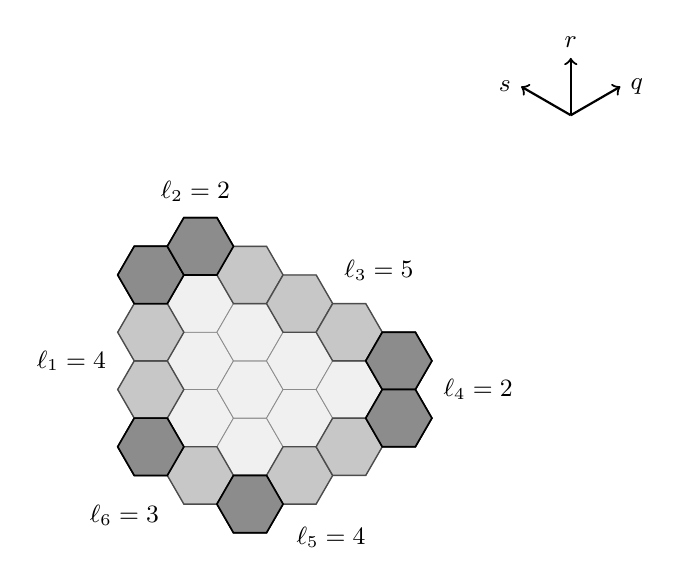
\begin{tikzpicture}[scale=0.42]
  \draw[fill=black!6,draw=black!45,line width=0.3pt] (1.000,3.464) -- (0.500,4.330) -- (-0.500,4.330) -- (-1.000,3.464) -- (-0.500,2.598) -- (0.500,2.598) -- cycle;
  \draw[fill=black!6,draw=black!45,line width=0.3pt] (1.000,5.196) -- (0.500,6.062) -- (-0.500,6.062) -- (-1.000,5.196) -- (-0.500,4.330) -- (0.500,4.330) -- cycle;
  \draw[fill=black!6,draw=black!45,line width=0.3pt] (1.000,6.928) -- (0.500,7.794) -- (-0.500,7.794) -- (-1.000,6.928) -- (-0.500,6.062) -- (0.500,6.062) -- cycle;
  \draw[fill=black!6,draw=black!45,line width=0.3pt] (1.000,8.660) -- (0.500,9.526) -- (-0.500,9.526) -- (-1.000,8.660) -- (-0.500,7.794) -- (0.500,7.794) -- cycle;
  \draw[fill=black!6,draw=black!45,line width=0.3pt] (2.500,2.598) -- (2.000,3.464) -- (1.000,3.464) -- (0.500,2.598) -- (1.000,1.732) -- (2.000,1.732) -- cycle;
  \draw[fill=black!6,draw=black!45,line width=0.3pt] (2.500,4.330) -- (2.000,5.196) -- (1.000,5.196) -- (0.500,4.330) -- (1.000,3.464) -- (2.000,3.464) -- cycle;
  \draw[fill=black!6,draw=black!45,line width=0.3pt] (2.500,6.062) -- (2.000,6.928) -- (1.000,6.928) -- (0.500,6.062) -- (1.000,5.196) -- (2.000,5.196) -- cycle;
  \draw[fill=black!6,draw=black!45,line width=0.3pt] (2.500,7.794) -- (2.000,8.660) -- (1.000,8.660) -- (0.500,7.794) -- (1.000,6.928) -- (2.000,6.928) -- cycle;
  \draw[fill=black!6,draw=black!45,line width=0.3pt] (2.500,9.526) -- (2.000,10.392) -- (1.000,10.392) -- (0.500,9.526) -- (1.000,8.660) -- (2.000,8.660) -- cycle;
  \draw[fill=black!6,draw=black!45,line width=0.3pt] (4.000,1.732) -- (3.500,2.598) -- (2.500,2.598) -- (2.000,1.732) -- (2.500,0.866) -- (3.500,0.866) -- cycle;
  \draw[fill=black!6,draw=black!45,line width=0.3pt] (4.000,3.464) -- (3.500,4.330) -- (2.500,4.330) -- (2.000,3.464) -- (2.500,2.598) -- (3.500,2.598) -- cycle;
  \draw[fill=black!6,draw=black!45,line width=0.3pt] (4.000,5.196) -- (3.500,6.062) -- (2.500,6.062) -- (2.000,5.196) -- (2.500,4.330) -- (3.500,4.330) -- cycle;
  \draw[fill=black!6,draw=black!45,line width=0.3pt] (4.000,6.928) -- (3.500,7.794) -- (2.500,7.794) -- (2.000,6.928) -- (2.500,6.062) -- (3.500,6.062) -- cycle;
  \draw[fill=black!6,draw=black!45,line width=0.3pt] (4.000,8.660) -- (3.500,9.526) -- (2.500,9.526) -- (2.000,8.660) -- (2.500,7.794) -- (3.500,7.794) -- cycle;
  \draw[fill=black!6,draw=black!45,line width=0.3pt] (5.500,2.598) -- (5.000,3.464) -- (4.000,3.464) -- (3.500,2.598) -- (4.000,1.732) -- (5.000,1.732) -- cycle;
  \draw[fill=black!6,draw=black!45,line width=0.3pt] (5.500,4.330) -- (5.000,5.196) -- (4.000,5.196) -- (3.500,4.330) -- (4.000,3.464) -- (5.000,3.464) -- cycle;
  \draw[fill=black!6,draw=black!45,line width=0.3pt] (5.500,6.062) -- (5.000,6.928) -- (4.000,6.928) -- (3.500,6.062) -- (4.000,5.196) -- (5.000,5.196) -- cycle;
  \draw[fill=black!6,draw=black!45,line width=0.3pt] (5.500,7.794) -- (5.000,8.660) -- (4.000,8.660) -- (3.500,7.794) -- (4.000,6.928) -- (5.000,6.928) -- cycle;
  \draw[fill=black!6,draw=black!45,line width=0.3pt] (7.000,3.464) -- (6.500,4.330) -- (5.500,4.330) -- (5.000,3.464) -- (5.500,2.598) -- (6.500,2.598) -- cycle;
  \draw[fill=black!6,draw=black!45,line width=0.3pt] (7.000,5.196) -- (6.500,6.062) -- (5.500,6.062) -- (5.000,5.196) -- (5.500,4.330) -- (6.500,4.330) -- cycle;
  \draw[fill=black!6,draw=black!45,line width=0.3pt] (7.000,6.928) -- (6.500,7.794) -- (5.500,7.794) -- (5.000,6.928) -- (5.500,6.062) -- (6.500,6.062) -- cycle;
  \draw[fill=black!6,draw=black!45,line width=0.3pt] (8.500,4.330) -- (8.000,5.196) -- (7.000,5.196) -- (6.500,4.330) -- (7.000,3.464) -- (8.000,3.464) -- cycle;
  \draw[fill=black!6,draw=black!45,line width=0.3pt] (8.500,6.062) -- (8.000,6.928) -- (7.000,6.928) -- (6.500,6.062) -- (7.000,5.196) -- (8.000,5.196) -- cycle;
  \draw[fill=black!22,draw=black!70,line width=0.5pt] (1.000,3.464) -- (0.500,4.330) -- (-0.500,4.330) -- (-1.000,3.464) -- (-0.500,2.598) -- (0.500,2.598) -- cycle;
  \draw[fill=black!22,draw=black!70,line width=0.5pt] (1.000,5.196) -- (0.500,6.062) -- (-0.500,6.062) -- (-1.000,5.196) -- (-0.500,4.330) -- (0.500,4.330) -- cycle;
  \draw[fill=black!22,draw=black!70,line width=0.5pt] (1.000,6.928) -- (0.500,7.794) -- (-0.500,7.794) -- (-1.000,6.928) -- (-0.500,6.062) -- (0.500,6.062) -- cycle;
  \draw[fill=black!22,draw=black!70,line width=0.5pt] (1.000,8.660) -- (0.500,9.526) -- (-0.500,9.526) -- (-1.000,8.660) -- (-0.500,7.794) -- (0.500,7.794) -- cycle;
  \draw[fill=black!22,draw=black!70,line width=0.5pt] (1.000,8.660) -- (0.500,9.526) -- (-0.500,9.526) -- (-1.000,8.660) -- (-0.500,7.794) -- (0.500,7.794) -- cycle;
  \draw[fill=black!22,draw=black!70,line width=0.5pt] (2.500,9.526) -- (2.000,10.392) -- (1.000,10.392) -- (0.500,9.526) -- (1.000,8.660) -- (2.000,8.660) -- cycle;
  \draw[fill=black!22,draw=black!70,line width=0.5pt] (2.500,9.526) -- (2.000,10.392) -- (1.000,10.392) -- (0.500,9.526) -- (1.000,8.660) -- (2.000,8.660) -- cycle;
  \draw[fill=black!22,draw=black!70,line width=0.5pt] (4.000,8.660) -- (3.500,9.526) -- (2.500,9.526) -- (2.000,8.660) -- (2.500,7.794) -- (3.500,7.794) -- cycle;
  \draw[fill=black!22,draw=black!70,line width=0.5pt] (5.500,7.794) -- (5.000,8.660) -- (4.000,8.660) -- (3.500,7.794) -- (4.000,6.928) -- (5.000,6.928) -- cycle;
  \draw[fill=black!22,draw=black!70,line width=0.5pt] (7.000,6.928) -- (6.500,7.794) -- (5.500,7.794) -- (5.000,6.928) -- (5.500,6.062) -- (6.500,6.062) -- cycle;
  \draw[fill=black!22,draw=black!70,line width=0.5pt] (8.500,6.062) -- (8.000,6.928) -- (7.000,6.928) -- (6.500,6.062) -- (7.000,5.196) -- (8.000,5.196) -- cycle;
  \draw[fill=black!22,draw=black!70,line width=0.5pt] (8.500,4.330) -- (8.000,5.196) -- (7.000,5.196) -- (6.500,4.330) -- (7.000,3.464) -- (8.000,3.464) -- cycle;
  \draw[fill=black!22,draw=black!70,line width=0.5pt] (8.500,6.062) -- (8.000,6.928) -- (7.000,6.928) -- (6.500,6.062) -- (7.000,5.196) -- (8.000,5.196) -- cycle;
  \draw[fill=black!22,draw=black!70,line width=0.5pt] (4.000,1.732) -- (3.500,2.598) -- (2.500,2.598) -- (2.000,1.732) -- (2.500,0.866) -- (3.500,0.866) -- cycle;
  \draw[fill=black!22,draw=black!70,line width=0.5pt] (5.500,2.598) -- (5.000,3.464) -- (4.000,3.464) -- (3.500,2.598) -- (4.000,1.732) -- (5.000,1.732) -- cycle;
  \draw[fill=black!22,draw=black!70,line width=0.5pt] (7.000,3.464) -- (6.500,4.330) -- (5.500,4.330) -- (5.000,3.464) -- (5.500,2.598) -- (6.500,2.598) -- cycle;
  \draw[fill=black!22,draw=black!70,line width=0.5pt] (8.500,4.330) -- (8.000,5.196) -- (7.000,5.196) -- (6.500,4.330) -- (7.000,3.464) -- (8.000,3.464) -- cycle;
  \draw[fill=black!22,draw=black!70,line width=0.5pt] (1.000,3.464) -- (0.500,4.330) -- (-0.500,4.330) -- (-1.000,3.464) -- (-0.500,2.598) -- (0.500,2.598) -- cycle;
  \draw[fill=black!22,draw=black!70,line width=0.5pt] (2.500,2.598) -- (2.000,3.464) -- (1.000,3.464) -- (0.500,2.598) -- (1.000,1.732) -- (2.000,1.732) -- cycle;
  \draw[fill=black!22,draw=black!70,line width=0.5pt] (4.000,1.732) -- (3.500,2.598) -- (2.500,2.598) -- (2.000,1.732) -- (2.500,0.866) -- (3.500,0.866) -- cycle;
  \draw[fill=black!45,draw=black,line width=0.6pt] (1.000,8.660) -- (0.500,9.526) -- (-0.500,9.526) -- (-1.000,8.660) -- (-0.500,7.794) -- (0.500,7.794) -- cycle;
  \draw[fill=black!45,draw=black,line width=0.6pt] (2.500,9.526) -- (2.000,10.392) -- (1.000,10.392) -- (0.500,9.526) -- (1.000,8.660) -- (2.000,8.660) -- cycle;
  \draw[fill=black!45,draw=black,line width=0.6pt] (8.500,6.062) -- (8.000,6.928) -- (7.000,6.928) -- (6.500,6.062) -- (7.000,5.196) -- (8.000,5.196) -- cycle;
  \draw[fill=black!45,draw=black,line width=0.6pt] (8.500,4.330) -- (8.000,5.196) -- (7.000,5.196) -- (6.500,4.330) -- (7.000,3.464) -- (8.000,3.464) -- cycle;
  \draw[fill=black!45,draw=black,line width=0.6pt] (4.000,1.732) -- (3.500,2.598) -- (2.500,2.598) -- (2.000,1.732) -- (2.500,0.866) -- (3.500,0.866) -- cycle;
  \draw[fill=black!45,draw=black,line width=0.6pt] (1.000,3.464) -- (0.500,4.330) -- (-0.500,4.330) -- (-1.000,3.464) -- (-0.500,2.598) -- (0.500,2.598) -- cycle;
  \node[font=\small] at (-2.40,6.06) {$ \ell_1=4 $};
  \node[font=\small] at (1.35,11.19) {$ \ell_2=2 $};
  \node[font=\small] at (6.90,8.79) {$ \ell_3=5 $};
  \node[font=\small] at (9.90,5.20) {$ \ell_4=2 $};
  \node[font=\small] at (5.45,0.73) {$ \ell_5=4 $};
  \node[font=\small] at (-0.80,1.40) {$ \ell_6=3 $};
  \draw[->,thick] (12.70,13.49) -- ++(1.5,0.866) node[right,font=\small] {$q$};
  \draw[->,thick] (12.70,13.49) -- ++(0,1.732) node[above,font=\small] {$r$};
  \draw[->,thick] (12.70,13.49) -- ++(-1.5,0.866) node[left,font=\small] {$s$};
\end{tikzpicture}

\caption{tight hull \(H(7;1,1,2)\)．六本の辺線を淡く，六つの隅セル
\(\kappa_{1},\dots,\kappa_{6}\) を濃く塗ってある．辺長は第~\ref{sec:2.3}~節の巡回順，すなわち
\(q_{\min}\)，\(r_{\max}\)，\(s_{\max}\)，\(q_{\max}\)，\(r_{\min}\)，\(s_{\min}\) の順に
\(\ell_{1},\dots,\ell_{6}\) である．ここでは \(\sum_{i}\ell_{i}=20=\lambda(H)+3\) であり，
三つの対辺差はいずれも \(\delta(H)=2\)，最短辺長は \(h=2\)．}\label{fig:hull}
\end{figure}

\begin{remark}[帰属]\label{rem:fs}
同値な defect 恒等式は，Fülep と Sieben による polyiamond の恒等式
\cite[Lemma~3.3]{FulepSieben2010} を，同論文の第 5 節で展開されている三角格子と六角格子の
双対を通して移すことで得られる．同じ site 周長の変数の下で，彼らの
\cite[Proposition~5.10]{FulepSieben2010} は，代入 \(p=t+3\) の後にちょうど
第~\ref{sec:capacity}~節の容量関数 \(M(t)\) を与える．そこで除外されている値 \(p=7\) は，下の
注意~\ref{rem:attain} で除外される値 \(t=4\) に対応する．それでも本稿では議論を自足的に保つ
ため辺周長変数で導出を与え，二つの設定を同一視しない．\cite{FulepSieben2010} は site 周長に
関するものである（注意~\ref{rem:site}）．
\end{remark}



\section{容量と最小辺周長}\label{sec:capacity}

\subsection{peeling と極値容量}\label{sec:2.6}

容量の計算が必要とする，方向凸な polyhex に対する二つの操作をまず記録する．support trace を
丸ごと取り除く操作と，それを一セルずつ戻す操作である．

\begin{lemma}[peeling]\label{lem:peel}
\(K\) を方向凸な polyhex，\(\Lambda\) をその六本の extreme line の一つ，
\(K':=K\sm\Lambda\) とする．\(K'\neq\emptyset\) ならば
\begin{enumerate}
\item[(i)] \(K'\) は方向凸な polyhex であって \(\sigma(K')\le\sigma(K)-1\)；
\item[(ii)] \(K\cap\Lambda\) のセルを \(c_{1},\dots,c_{k}\) と順序づけて，各 \(j\) について
\(K'\cup\{c_{1},\dots,c_{j}\}\) が辺半周長 \(\sigma(K)\) 以下の方向凸な polyhex になるように
できる．
\end{enumerate}
\end{lemma}

\begin{proof}
\(\Lambda\) を線 \(q=q_{\min}\) とする．他の五つの場合も，鍵の役割と各族の二つの向きを入れ替え
れば同じである．

(i) \(q\) の占有値 \(k\) ごとに \(K_{k}\) を線 \(q=k\) 上の \(K\) のトレースとすると，これは
run である．\(K\) は連結だから，連続する値 \(k,k+1\) について \(K_{k}\) のセルと \(K_{k+1}\) の
セルを結ぶ \(K\) 内の道が存在し，事実~\ref{f:3} によりその道は \(q=k\) のセルから \(q=k+1\) の
セルへの一歩を含む．したがって \(K_{k}\) と \(K_{k+1}\) は隣接する．ゆえに
\(k\ge q_{\min}+1\) なる \(K_{k}\) の合併である \(K'\) は連結である．\(q\)-族における \(K'\) の
トレースは \(K\) のトレースそのものだから run である．次に \(r\)-族の線 \(r=k\) を固定する．
そのセルは \((q,k)\) で表されるから，この線上の \(K\) のトレースが run であることは，そこでの
\(q\) の値が整数区間をなすことと同値である．事実~\ref{f:2} によりこの線は \(\Lambda\) と
高々一セル \((q_{\min},k)\) で交わる．\(K'\) のトレースは，存在するならこのセルだけを
\(K\) のトレースから除いたものである．\(q_{\min}\) は \(K\) 全体で最小の \(q\) 値だから，
この整数区間の最小値であり，それを除いても空集合または整数区間が残る．
\(s\)-族の線 \(s=k\) もセルを \((q,k-q)\) として同じく \(q\) で媒介でき，全く同じ議論が
成り立つ．よって \(K'\) のすべてのトレースは run であり，\(K'\) は方向凸である．最後に
\(\Lambda\) は \(K\) に占有されて \(K'\) には占有されないから \(\lambda(K')\le\lambda(K)-1\) であり，補題~\ref{lem:runs} より
\(\sigma(K')=\lambda(K')\le\lambda(K)-1=\sigma(K)-1\)．

(ii) \(K\) は連結だから \(K'\) に隣接するセル \(c_{1}\in K\cap\Lambda\) が存在する．run
\(K\cap\Lambda\) の残りのセルを，どの先頭部分 \(\{c_{1},\dots,c_{j}\}\) も \(c_{1}\) を含む
連続ブロックになるように順序づける．\(K_{j}:=K'\cup\{c_{1},\dots,c_{j}\}\) と書く．
\(c_{1}\) は \(K'\) に隣接し，以後の各 \(c_{j}\) は既に入れたセルに隣接するから \(K_{j}\) は
連結である．\(\Lambda\) 上のトレースはブロックなので run であり，\(q\)-族の他の線上の
トレースは \(K'\) のトレースそのものである．\(r\)-族または \(s\)-族の線では，(i) と同様に
\(q\) で媒介すると，\(K_j\) のトレースは \(K'\) のトレースに高々一つの挿入セルを加えたもの
である．そのセルは \(\Lambda\) 上にあり \(q=q_{\min}\) を持つ．\(K\) のトレースはこのセルを
含む run であり，(i) により \(K'\) のトレースはその run から最小要素 \(q_{\min}\) を除いたもの
だから，セルを戻すと \(K\) の run が復元される．よって \(K_j\) のすべてのトレースは run で，
\(K_j\) は方向凸である．\(K_j\) が占有する線はすべて \(K\) が占有するから
\(\sigma(K_{j})=\lambda(K_{j})\le\lambda(K)=\sigma(K)\)．
\end{proof}

\begin{corollary}\label{cor:subsets}
\(K\) を方向凸な polyhex とする．\(1\le j\le|K|\) なる各 \(j\) について，方向凸な polyhex
\(K_{j}\subseteq K\) であって \(|K_{j}|=j\) かつ \(\sigma(K_{j})\le\sigma(K)\) なるものが存在
する．
\end{corollary}

\begin{proof}
\(|K|\) に関する強帰納法．\(|K|=1\) なら自明．\(|K|\ge2\) とする．ある extreme line
\(\Lambda\) は \(K\) の全体を含まない．さもなくば \(K\) は異なる族の二本の extreme line に
含まれることになり，事実~\ref{f:2} によりそれらは一セルでしか交わらないから \(|K|\ge2\) に
矛盾する．その \(\Lambda\) に補題~\ref{lem:peel} を適用する．(ii) の集合 \(K_{j}\) が
\(|K'|\) から \(|K|\) までのすべてのサイズを与え，\(|K'|\) 未満のサイズは，辺半周長が
\(\sigma(K)\) 以下である \(K'\) に帰納法の仮定を適用して得られる．
\end{proof}

\begin{definition}\label{def:M}
整数 \(t\ge0\) に対し
\[
   M(t):=\left\lfloor\frac{t^{2}+3}{12}\right\rfloor
\]
とおく．言葉では，\(t\) の平方に 3 を加えたものの 12 分の 1 の整数部分である．したがって
\(M(0)=M(1)=M(2)=0\)，\(M(3)=1\)．関数 \(M\) は単調非減少である．
\end{definition}

\begin{theorem}\label{thm:capacity}
\(N\ge1\) とする．
\begin{enumerate}
\item[(a)] 任意の polyhex \(S\) は \(|S|\le M(\sigma(S))\) を満たす．言葉では，辺半周長が
\(t\) の配置は \(M(t)\) より多くのセルを持てない．
\item[(b)] 各 \(t\ge3\) に対し，方向凸な polyhex \(K\) であって \(|K|=M(t)\) かつ
\(\sigma(K)\le t\) なるものが存在する．
\item[(c)] \(N\) セル polyhex の最小辺周長は
\[
   p_{\min}(N)=2g(N),\qquad g(N)=\left\lceil\sqrt{12N-3}\,\right\rceil
\]
である．言葉では，\(N\) セルを収容できる最小の辺半周長は，12 倍の \(N\) から 3 を引いたものの
平方根以上の最小の整数であり，最小辺周長はその 2 倍である．
\item[(d)] 任意の \(N\) セル最小配置 \(S\) は方向凸であって
\(\sigma(S)=\lambda(S)=g(N)\) を満たす．
\end{enumerate}
\end{theorem}

(d) の最小配置の方向凸性は既知結果でもある．Davoli, Piovano, Stefanelli
\cite[Definition~3.2 and Proposition~3.3]{DavoliPiovanoStefanelli2017} は三角格子上の辺等周問題
のすべての最小配置が \emph{3-convex}，すなわち同じ格子線上の二点の間にある全格子点を含むこと
を示している．第~\ref{sec:0.5}~節の同一視の下で，これは本稿の方向凸性そのものである．彼らは
平行線上の点数を並べ替える rearrangement により証明するが，以下では hull 恒等式と容量上界から
(d) を導き，同時に以後必要な \(\lambda(S)=g(N)\) まで得る．方向凸性自体の新しい証明を主張する
ためではなく，本稿を自足的にするため全文を残す．

\begin{proof}
(a) \(H=H(S)\) とする．補題~\ref{lem:hull} と補題~\ref{lem:hex}(v) より
\[
   12|S|\le12|H|=\lambda(H)^{2}+3-\bigl(3\delta(H)^{2}+2Q(H)\bigr)\le\lambda(S)^{2}+3
   \le\sigma(S)^{2}+3 ,
\]
最後の段は補題~\ref{lem:runs} による．\(|S|\) は整数だから \(|S|\le M(\sigma(S))\)．

(b) \(t\equiv3\pmod 6\)，たとえば \(t=6m+3\) のときは \(K=H(3m+1;m,m,m)\) を取る．\(t=6m\) の
ときは \(H(3m-1;m-1,m-1,m-1)\)，\(t=6m+1\) のときは \(H(3m;m,m,m-1)\)，\(t=6m+2\) のときは
\(H(3m+1;m,m,m+1)\)，\(t=6m+4\) のときは \(H(3m+1;m,m,m-1)\)，\(t=6m+5\) のときは
\(H(3m+2;m,m,m+1)\) を取る．ここで \(t\equiv3,5\pmod6\) では \(m\ge0\)，
残る四つの剰余では \(m\ge1\) であり，これで \(t=4\) を除くすべての \(t\ge3\) を覆う．
いずれの場合も \eqref{eq:adm} が成り立ち，
補題~\ref{lem:hex}(ii) より \(\sigma(K)=t\)，補題~\ref{lem:hex}(iv),(v) より
\(12|K|=t^{2}+3-D\) であって \(t\) の剰余に応じて \(D\in\{0,3,4,7\}\) となるから
\(|K|=M(t)\)．許容的な三つ組で覆われない唯一の場合は \(t=4\) であり，そこでは \(M(4)=1\) で
あって単一セルの辺半周長は \(3\le4\) である．

(c) \(t_{N}:=\min\{t\ge3:\ M(t)\ge N\}\) とおく．(a) より任意の \(N\) セル polyhex は
\(M(\sigma(S))\ge N\) を満たすから \(\sigma(S)\ge t_{N}\)．逆に (b) は \(|K|=M(t_{N})\ge N\)
かつ \(\sigma(K)\le t_{N}\) なる方向凸 \(K\) を与え，系~\ref{cor:subsets} がそこから辺半周長
\(t_{N}\) 以下の \(N\) セル polyhex を取り出す．よって \(p_{\min}(N)=2t_{N}\)．最後に整数
\(t\) に対し
\[
   M(t)\ge N\iff \frac{t^{2}+3}{12}\ge N\iff t\ge\sqrt{12N-3},
\]
であり \(N\ge1\) では \(\sqrt{12N-3}\ge3\) だから \(t_{N}=g(N)\)．

(d) (c) より \(\sigma(S)=g(N)\)．\(H=H(S)\) とする．\(H\) は方向凸で
\(\sigma(H)=\lambda(H)\) だから (a) を \(H\) に適用して \(M(\lambda(H))\ge|H|\ge N\)，したがって
\(\lambda(H)\ge t_{N}=g(N)\)．補題~\ref{lem:runs} と補題~\ref{lem:hull} と合わせて
\[
   g(N)=\sigma(S)=R(S)\ \ge\ \lambda(S)=\lambda(H)\ \ge\ g(N)
\]
となるから \(R(S)=\lambda(S)\)，すなわち \(S\) は方向凸である．
\end{proof}

\begin{remark}\label{rem:attain}
(a) と (b) を合わせると，ちょうど
\[
   M(t)=\max\{\,|K|:\ K\text{ は }\sigma(K)\le t\text{ なる polyhex}\,\}
\]
である．言葉では，\(M(t)\) とは辺半周長の予算 \(t\) の中に収まる最大のセル数である．本稿の
以降が用いるのはこの予算形であり，(b) の不等号は弱めではない．\(t=4\) を除く各 \(t\ge3\) に
ついて証明中の六角形は実際に \(\sigma(K)=t\) を満たし，\(t=4\) はそもそもどの polyhex の辺半
周長でもない．実際 \(\sigma(K)=4\) なる polyhex \(K\) は (a) より \(|K|\le M(4)=1\) となるが，
一セルの polyhex の辺半周長は 3 である．
\end{remark}

\subsection{plateau の橋渡し}\label{sec:2.7}

関数 \(N\mapsto g(N)\) は単調非減少であり，各値を連続する整数のブロック上で取る．\(g\) の値域
に属する \(\gamma\) に対し
\[
   N_{b}(\gamma):=\min\{\,N\ge1:\ g(N)=\gamma\,\}
\]
を，最小辺半周長が \(\gamma\) に等しくなる最初のセル数とする．

\begin{lemma}\label{lem:bridge}
\(g\) の値域に属する任意の \(\gamma\) について
\begin{equation}\label{eq:bridge}
   N_{b}(\gamma)=M(\gamma-1)+1 ,
\end{equation}
言葉では，最小辺半周長が \(\gamma\) となる plateau は，辺半周長 \(\gamma-1\) の容量を使い切った
一つ先のセル数から始まる．
\end{lemma}

\begin{proof}
整数 \(N\ge1\) と \(t\ge3\) について，定理~\ref{thm:capacity}(c) の証明と同様に，
\(g(N)\le t\) と \(N\le M(t)\) は同値である．したがって
\(\{N:\ g(N)\le\gamma-1\}=\{1,\dots,M(\gamma-1)\}\) であり，\(g(N)\ge\gamma\) なる最小の \(N\)
は \(M(\gamma-1)+1\) である．\(\gamma\) が \(g\) の値域に属するから，その最小の \(N\) は
\(g(N)=\gamma\) を満たす．
\end{proof}

補題~\ref{lem:bridge} は第~\ref{sec:skeleton}~節で，最小配置が plateau の開始点にあることを
認識するために用いる．


\section{最短辺と，例外的な plateau 開始点における剛性}\label{sec:rigidity}

本節を通じて \(S\) を辺周長最小配置，\(n=|S|\)，\(\sigma=\sigma(S)=g(n)\) とする．
定理~\ref{thm:capacity}(d) より \(S\) は方向凸なので support trace \(r_{i}\) と
\(\rho(S)=\min_{i}r_{i}\) が定義され，補題~\ref{lem:hull}(iii) より \(\rho(S)\ge1\)．
\(H=H(S)\) とする．

以下では四つの用語を区別する．\(S\) の六本の \emph{extreme line}
\(\Lambda_i\)（第~\ref{sec:2.3}~節）は，補題~\ref{lem:hull}(ii) により \(H\) の六本の
\emph{辺線}と同じ線である．各線上には，長さ \(\ell_i\) の hull の\emph{辺}
\(H\cap\Lambda_i\) と，長さ \(r_i\) の配置の\emph{support trace}
\(S\cap\Lambda_i\) がある．\emph{最短辺}は \(h=\min_i\ell_i\) を指し，
\emph{最短 extreme line} または \emph{最短 support trace} は
\(\rho(S)=\min_i r_i\) を指す．第~\ref{sec:skeleton}~節の定理が削除するのは最短 support
trace であり，以下の剛性議論はそれを hull の辺と比較する．

\begin{observation}\label{obs:fullside}
\(S\) を方向凸な polyhex，\(H\) をその tight hull とする．
\begin{enumerate}
\item[(a)] 各 \(i\) について \(S\cap\Lambda_i\subseteq H\cap\Lambda_i\) だから
\(r_i\le\ell_i\)．また \(r_i=\ell_i\) と
\(S\cap\Lambda_i=H\cap\Lambda_i\)，すなわち hull の辺全体が \(S\) に含まれることは同値である．
\item[(b)] \(H\cap\Lambda_i\) に巡回順で隣接する二辺
\(H\cap\Lambda_{i-1}\)，\(H\cap\Lambda_{i+1}\) がともに \(S\) に含まれるなら，
\(H\cap\Lambda_i\) も \(S\) に含まれる．
\end{enumerate}
\end{observation}

\begin{proof}
(a) は補題~\ref{lem:hull}(i) を \(\Lambda_i\) に制限したもの．包含関係にある二つの有限集合は
濃度が等しいとき，かつそのときに限り一致する．(b) について，隅
\(\kappa_{i-1}=H\cap\Lambda_{i-1}\cap\Lambda_i\) と
\(\kappa_i=H\cap\Lambda_i\cap\Lambda_{i+1}\) は，仮定した二つの完全な辺上にあるから
\(S\) に属する．補題~\ref{lem:hex}(i) によりこれらは run \(H\cap\Lambda_i\) の両端セルで
あり，\(S\cap\Lambda_i\) はその両端を含む run だから辺全体を含む．
\end{proof}

\begin{lemma}\label{lem:rhobound}
\(\displaystyle \rho(S)\le\Bigl\lfloor\frac{\sigma+3}{6}\Bigr\rfloor\)．言葉では，最短の
support trace は \(\sigma+3\) の六分の一以下のセルしか持たない．
\end{lemma}

\begin{proof}
補題~\ref{lem:hull}(ii) と \eqref{eq:sidesum} より \(\sum_{i}\ell_{i}=\lambda(H)+3=\sigma+3\)．
\(S\subseteq H\) より \(r_{i}\le\ell_{i}\) だから \(\sum_{i}r_{i}\le\sigma+3\)．六つの整数の
最小値はその平均以下である．
\end{proof}

この上界は，六辺ができる限り等しい hull で達成され，それがまさに，ある種の plateau の開始点で
起こることである．次の命題は本稿で唯一の微妙な段階であり，そのような plateau 開始点では最小
配置の六つの support trace がすべてそれほど長くはなれないことを述べる．

\begin{proposition}[例外的な plateau 開始点における剛性]\label{pro:rigidity}
\(m\ge1\) とし，\(\gamma\) を \(g\) の値域に属し \(\gamma\in\{6m+3,\ 6m+5\}\) なるものとし，
\(S\) を \(|S|=N_{b}(\gamma)\) なる辺周長最小配置とする．このとき \(\rho(S)\le m\)．
\end{proposition}

言葉では，閾値が 6 を法として 3 または 5 である plateau の開始点では，最小配置の最短
support trace は補題~\ref{lem:rhobound} の上界（ここでは \(m+1\)）より真に短い．

\begin{proof}
\(N=N_{b}(\gamma)\) とおく．補題~\ref{lem:bridge} より \(N=M(\gamma-1)+1\) であり，二つの剰余
について
\begin{equation}\label{eq:nbspecial}
   N_{b}(6h-3)=3h^{2}-4h+2,\qquad N_{b}(6h-1)=3h^{2}-2h+1\qquad(h=m+1)
\end{equation}
を得る．\(\bigl((6h-4)^{2}+3\bigr)/12\) の整数部分は \(3h^{2}-4h+1\)，
\(\bigl((6h-2)^{2}+3\bigr)/12\) の整数部分は \(3h^{2}-2h\) だからである．
定理~\ref{thm:capacity}(d) より \(S\) は方向凸で \(\lambda(S)=\gamma\)，したがって
補題~\ref{lem:hull}(ii) より \(\lambda(H)=\gamma\)．

\medskip\noindent\textbf{場合 \(\gamma\equiv3\pmod6\)．} \(\gamma=6h-3\) と書くと \(h=m+1\ge2\)．
\(\rho(S)\le h-1\) を示せばよい．\(\rho(S)\ge h\) と仮定する．すると各 support trace が \(h\)
セル以上を持つから hull の各辺は \(\ell_{i}\ge r_{i}\ge h\) を満たす．\eqref{eq:sidesum} と
補題~\ref{lem:hull}(ii) より \(\sum_{i}\ell_{i}=\gamma+3=6h\) だから，六辺すべてがちょうど \(h\)
である．\(\ell_{2}=v+1=\ell_{4}=u+1=\ell_{6}=w+1=h\) と \(\ell_{1}=L-v-w=h\) を解くと
\[
   u=v=w=h-1,\qquad L=3h-2,
\]
したがって補題~\ref{lem:hex}(iv) より
\[
   |H|=T(3h-2)-3\,T(h-1)=3h^{2}-3h+1 .
\]
\eqref{eq:nbspecial} より \(N=3h^{2}-4h+2\) だから \(|H|-N=h-1\ge1\)．しかしすべての \(i\) について \(r_i\ge h=\ell_i\) であることは，
観察~\ref{obs:fullside}(a) により hull の各辺が丸ごと \(S\) に含まれることを意味する．
補題~\ref{lem:complete} より \(S=H\) となり，\(|S|=N<|H|\) に矛盾する．

\medskip\noindent\textbf{場合 \(\gamma\equiv5\pmod6\)．} \(\gamma=6h-1\) と書くと，やはり
\(h=m+1\ge2\)．\(\rho(S)\ge h\) と仮定する．前と同様に各辺は \(\ell_{i}\ge h\) を満たし，今度は
\(\sum_{i}\ell_{i}=\gamma+3=6h+2\) だから，最短辺の長さはちょうど \(h\) で \(\sum_{i}x_{i}=2\)．補題~\ref{lem:oppair} より
ちょうど一組の対辺が長さ \(h+1\) を持つ．格子の \(120^{\circ}\) 回転は三つの族を巡回的に
入れ替え，polyhex を polyhex に写し，隣接・周長・六本の extreme line の集合を保存し，\(S\) の
tight hull を回転後の \(S\) の tight hull に写す（回転後に定義~\ref{def:hull} の正規化を
改めて行う）．したがってその組が \(q\)-族の二辺 \((\ell_1,\ell_4)\) であるとしてよい．
\(\ell_{4}=u+1=h+1\)，\(\ell_{2}=v+1=h\)，\(\ell_{6}=w+1=h\)，\(\ell_{1}=L-v-w=h+1\) を解くと
\[
   u=h,\qquad v=w=h-1,\qquad L=3h-1
\]
（\(\ell_{3}=\ell_{5}=h\) と \(\lambda(H)=3L-(u+v+w)=6h-1=\gamma\) を確かめられる），そして
\[
   |H|=T(3h-1)-T(h)-2\,T(h-1)=3h^{2}-h .
\]
\eqref{eq:nbspecial} より \(N=3h^{2}-2h+1\) だから，やはり \(|H|-N=h-1\ge1\)．

\(r_i\ge h\) と観察~\ref{obs:fullside}(a) から，長さ \(h\) の四辺
\(H\cap\Lambda_i\)（\(i=2,3,5,6\)）はすべて \(S\) に含まれる．長辺
\(H\cap\Lambda_1\) は巡回順で \(H\cap\Lambda_6\)，\(H\cap\Lambda_2\) に隣接し，両方とも
\(S\) に含まれるから，観察~\ref{obs:fullside}(b) より \(H\cap\Lambda_1\) も \(S\) に含まれる．
対辺 \(H\cap\Lambda_4\) も \(H\cap\Lambda_3\)，\(H\cap\Lambda_5\) から同様に従う．
よって六辺すべてが \(S\) に含まれ，補題~\ref{lem:complete} より \(S=H\) となって \(|S|=N<|H|\) に矛盾
する．
\end{proof}

次節における命題~\ref{pro:rigidity} の論理的役割は整数一単位だけである．
補題~\ref{lem:rhobound} と \(n\ge M(\sigma-1)+1\) という計数だけで，最短 support trace
\(\rho\) を削除した後のセル数について，\(\sigma\bmod6\) の四つの剰余類では
\(n-\rho\ge M(\sigma-2)+1\) が得られるが，\(\sigma\equiv3,5\pmod6\) では
\(n-\rho\ge M(\sigma-2)\) までしか出ない．等号が起こりうるのは plateau の開始点で
\(\rho=m+1\) の場合に限られる．命題はこの等号の場合を排除し，その二つの剰余類でも
\(n-\rho\ge M(\sigma-2)+1\) へ一単位引き上げる．この一単位によって，
定理~\ref{thm:skel} の段階 4 で剥ぎ取った配置が最小配置になる．

\section{最短辺 skeleton 定理}\label{sec:skeleton}

\begin{theorem}[最短辺 skeleton；定理~\ref{thm:intro-skel}]\label{thm:skel}
\(S\) を \(n=|S|\ge3\) の辺周長最小配置，\(\sigma=\sigma(S)=g(n)\) とし，\(\Lambda\) を
\(|S\cap\Lambda|=\rho(S)\) なる \(S\) の\emph{任意の} extreme line とする．
\(S':=S\sm\Lambda\) とおく．このとき
\begin{enumerate}
\item[(i)] \(S'\) は空でなく，\(g(|S'|)=\sigma-1\) なる辺周長最小配置である；
\item[(ii)] \(S\cap\Lambda\) のセルを \(c_{1},\dots,c_{\rho}\) と順序づけて，各
\(T_{j}:=S'\cup\{c_{1},\dots,c_{j}\}\) が \(\exc(T_{j})\le2\) なる方向凸 polyhex となるように
できる．
\end{enumerate}
\end{theorem}

言葉では，最小配置から最短 extreme line を剥ぐと閾値が一段下の最小配置に着地し，その線を
一セルずつ戻す途中の代価は辺周長 2 単位を超えない．

\begin{proof}
定理~\ref{thm:capacity}(d) より \(S\) は方向凸で \(\lambda(S)=\sigma\)，また
\(\rho=\rho(S)\ge1\)．\(n\ge3\)，\(g(3)=\lceil\sqrt{33}\rceil=6\)，\(g\) が単調非減少である
ことから \(\sigma\ge6\)．\(\sigma=6m+s\)，\(0\le s\le5\) と書くと \(m\ge1\)．

\medskip\noindent\textbf{段階 1（二つの上下界）．}
補題~\ref{lem:rhobound} より \(\rho\le\lfloor(\sigma+3)/6\rfloor\)．また \(g(n)=\sigma\) は
\(n>M(\sigma-1)\) を意味し，すなわち
\begin{equation}\label{eq:nbound}
   n\ \ge\ M(\sigma-1)+1 .
\end{equation}

\medskip\noindent\textbf{段階 2（剰余表）．}
\(t=6m+j\)，\(0\le j\le5\) に対し \(M(t)=3m^{2}+mj+\lfloor(j^{2}+3)/12\rfloor\) であり，
\(\lfloor(j^{2}+3)/12\rfloor\) は \(j=0,\dots,5\) について \(0,0,0,1,1,2\)．差を取り
（\(s=0\) では \(\sigma-1,\sigma-2\) の両方が，\(s=1\) では \(\sigma-2\) が
一つ前のブロック \(6(m-1)+j\) に落ちる），
\(\lfloor(\sigma+3)/6\rfloor=m+\lfloor(s+3)/6\rfloor\) を用いると次の表を得る．

\begin{center}
\begin{tabular}{crrr}
\hline
\(s=\sigma\bmod 6\) & \(M(\sigma-1)-M(\sigma-2)\) & \(\lfloor(\sigma+3)/6\rfloor\) & 差 \\
\hline
0 & \(m\)   & \(m\)   & \(0\) \\
1 & \(m\)   & \(m\)   & \(0\) \\
2 & \(m\)   & \(m\)   & \(0\) \\
3 & \(m\)   & \(m+1\) & \(-1\) \\
4 & \(m+1\) & \(m+1\) & \(0\) \\
5 & \(m\)   & \(m+1\) & \(-1\) \\
\hline
\end{tabular}
\end{center}

段階 1 の二つを合わせて \(n-\rho\ge M(\sigma-1)+1-\lfloor(\sigma+3)/6\rfloor\)．
\(s\notin\{3,5\}\) なら表より \(M(\sigma-1)-\lfloor(\sigma+3)/6\rfloor\ge M(\sigma-2)\) だから
\begin{equation}\label{eq:strict}
   n-\rho\ \ge\ M(\sigma-2)+1 .
\end{equation}
\(s\in\{3,5\}\) なら表は \(n-\rho\ge M(\sigma-2)\) しか与えず，等号は \eqref{eq:nbound} と
補題~\ref{lem:rhobound} が同時に等号になるとき，すなわち \(n=M(\sigma-1)+1\) かつ
\(\rho=m+1\) のときに限る．言葉では，厳密不等式 \eqref{eq:strict} が失敗しうるのは，閾値が
6 を法として 3 または 5，配置がその plateau のまさに先頭，最短トレースが数え上げの許す最大長，
という三つが同時に起こる場合だけである．

\medskip\noindent\textbf{段階 3（例外の場合は剛性で排除される）．}
\(s\in\{3,5\}\)，\(n=M(\sigma-1)+1\)，\(\rho=m+1\) と仮定する．補題~\ref{lem:bridge} より
\(n=N_{b}(\sigma)\)．また \(\sigma=g(n)\) は \(g\) の値域に属し，\(m\ge1\)．したがって
命題~\ref{pro:rigidity} が \(\gamma=\sigma\) について適用でき \(\rho\le m\) を与えるが，これは
\(\rho=m+1\) に矛盾する．ゆえに \eqref{eq:strict} はすべての剰余で成り立つ．

\medskip\noindent\textbf{段階 4（結論 (i)）．}
\eqref{eq:strict} と \(g\) の定義より \(g(n-\rho)\ge\sigma-1\)．
\(n-\rho\ge M(\sigma-2)+1\ge1\) だから \(S'\) は空でなく，補題~\ref{lem:peel}(i) が適用でき
る．すなわち \(S'\) は \(\sigma(S')\le\sigma-1\) なる方向凸 polyhex である．
補題~\ref{lem:runs} と定理~\ref{thm:capacity}(c) より
\[
   2(\sigma-1)\ \le\ 2g(|S'|)\ =\ p_{\min}(|S'|)\ \le\ p(S')\ =\ 2\sigma(S')\ \le\ 2(\sigma-1),
\]
よってすべて等号であり，\(S'\) は最小配置で \(g(|S'|)=\sigma-1\)．ここまでどの最短線
\(\Lambda\) を選んだかには依存していない．

\medskip\noindent\textbf{段階 5（結論 (ii)）．}
補題~\ref{lem:peel}(ii) より \(S\cap\Lambda\) の順序づけ \(c_{1},\dots,c_{\rho}\) であって，各
\(T_{j}\) が \(\sigma(T_{j})\le\sigma\) なる方向凸 polyhex になるものが存在する．
\(|T_{j}|\ge|S'|\) と \(g\) の単調性より \(g(|T_{j}|)\ge\sigma-1\)．したがって
\[
   \exc(T_{j})=p(T_{j})-2g(|T_{j}|)=2\bigl(\sigma(T_{j})-g(|T_{j}|)\bigr)
   \le2\bigl(\sigma-(\sigma-1)\bigr)=2 .
\]
言葉では，復元の途中で周長は出発時の値を超えない一方，閾値は既に一段下がっているので，超過は
高々 2 である．
\end{proof}

\begin{corollary}[骨格列]\label{cor:skel}
任意の辺周長最小配置 \(S\) は，辺周長最小配置の鎖
\(S=T_{0}\supset T_{1}\supset\cdots\supset T_{k}\)，\(|T_{k}|\le2\) であって，各々が直前の
ものから最短 extreme line を一本削除して得られ，各段で \(g(|T_{i+1}|)=g(|T_{i}|)-1\) となる
ものを持つ．
\end{corollary}

\begin{proof}
\(|T_{i}|\ge3\) の間，定理~\ref{thm:skel}(i) を適用する．サイズは厳密に減少する．
\end{proof}

\begin{proof}[定理~\ref{thm:intro-main} の証明]
系~\ref{cor:skel} の鎖を取る．\(|T_{k}|=2\) なら \(T_{k}\) はドミノで \(\exc=0\)，その一方の
セルは \(\exc=0\) の単一セルなので，鎖を一段延ばす．連続する二項の間に定理~\ref{thm:skel}(ii)
の配置 \(T_{j}\) を挿入する．各々は超過 2 以下の polyhex である．得られた列を単一セルから
\(S\) まで読めば (b) を得る．(a) については，各 \(S_{k+1}=S_{k}\cup\{c\}\) は連結で \(S_{k}\)
は空でないから \(c\) は \(S_{k}\) に隣接するセルを持つ．さもなくば \(\{c\}\) だけが
\(S_{k+1}\) の連結成分になる．
\end{proof}

\begin{remark}[手続き]\label{rem:algorithm}
構成は短く述べられる．最短 extreme line を繰り返し削除し，得られた最小配置の列を逆向きに
読んで，削除した各線を，残っている配置に隣接するセルから始めて一セルずつ戻す．最小配置
そのものが成長の骨格をなし，超過 2 は一本の線の復元の内部でだけ消費される．
\end{remark}


\section{定数 2 の最適性}\label{sec:sharp}

系~\ref{cor:skel} は，成長の骨格——一本の extreme line がちょうど復元された時点の配置——を
常に最小配置だけからなるように取れることを述べる．本節は，途中の一セル段階には同じことを
要求できないことを示す．すなわち定理~\ref{thm:intro-main} の定数 2 は下げられない．議論は
自足的で計算を用いない．一セル削除の効果に関する一つの恒等式を，明示的な一つの 13 セル最小
配置に適用する．

\subsection{削除の恒等式}\label{sec:8.1}

有限セル集合 \(S\) と \(c\in S\) について，\(S\) の中で \(c\) に隣接するセルの個数を
\(\dg_{S}(c)\) と書く．

\begin{lemma}\label{lem:deldeg}
任意の有限セル集合 \(S\) と任意の \(c\in S\) について
\begin{equation}\label{eq:deldeg}
   p(S\sm\{c\})=p(S)-6+2\dg_{S}(c).
\end{equation}
言葉では，一セルを取り除くとそのセルの六辺が境界から消える一方，そのセルが \(S\) の内側に持って
いた隣接ごとに，共有していた辺の両側が境界に戻ってくる．
\end{lemma}

\begin{proof}
\(n=|S|\)，\(a=a(S)\) と書く．\(c\) を削除すると一セルとちょうど \(\dg_{S}(c)\) 個の隣接対が
消えるから \(|S\sm\{c\}|=n-1\) かつ \(a(S\sm\{c\})=a-\dg_{S}(c)\)．定義
\(p(K)=6|K|-2a(K)\) より
\[
   p(S\sm\{c\})=6(n-1)-2\bigl(a-\dg_{S}(c)\bigr)=\bigl(6n-2a\bigr)-6+2\dg_{S}(c),
\]
これが \eqref{eq:deldeg} である．
\end{proof}

補題~\ref{lem:deldeg} で連結性は仮定していない．\eqref{eq:deldeg} は任意の有限セル集合に対する
恒等式である．連結性が問題になるのは，\(S\sm\{c\}\) を成長列における \(S\) の直前の配置として
使うときだけである．成長列は polyhex からなるからである．

\subsection{明示的な 13 セル最小配置}\label{sec:8.2}

\begin{example}\label{ex:13}
\[
   S^{\ast}:=\{(0,r):1\le r\le4\}\ \cup\ \{(1,r):0\le r\le4\}\ \cup\ \{(2,r):0\le r\le3\}
\]
とする．言葉では，連続する三本の \(q\)-線にそれぞれ 4，5，4 セルを置き，各々を run とし，全体
が polyhex になるように配置したものである．
\end{example}

\begin{lemma}\label{lem:13min}
\(S^{\ast}\) は方向凸な polyhex であって
\[
   |S^{\ast}|=13,\qquad p(S^{\ast})=26=p_{\min}(13),
\]
したがって 13 セルの最小配置である．その次数分布は
\[
   3^{6}\,4^{4}\,6^{3},
\]
言葉では，次数 3 のセルが 6 個，次数 4 が 4 個，次数 6 が 3 個であり，特に次数 2 以下のセルは
存在しない．
\end{lemma}

\begin{proof}
\(q\)-族の三つのトレースは run \(r\in[1,4]\)，\(r\in[0,4]\)，\(r\in[0,3]\) であり
\(|S^{\ast}|=4+5+4=13\)．\(r\)-族のトレースは
\[
   r=0:\ q\in[1,2],\quad r=1,2,3:\ q\in[0,2],\quad r=4:\ q\in[0,1],
\]
\(s\)-族のトレースは \(q\) の順に
\[
   s=1:\ q\in[0,1],\quad s=2,3,4:\ q\in[0,2],\quad s=5:\ q\in[1,2].
\]
すべてのトレースが単一の run だから \(S^{\ast}\) は方向凸であり，連続する \(q\)-トレースの
\(r\)-範囲が重なるから連結である．占有線を数えると \(\lambda(S^{\ast})=3+5+5=13\) であり，
補題~\ref{lem:runs} より \(p(S^{\ast})=2\lambda(S^{\ast})=26\)．\(12\cdot13-3=153\) かつ
\(12^{2}<153\le13^{2}\) だから \(g(13)=13\)，\(p_{\min}(13)=26\)．

次数について，三つのセル \((1,1),(1,2),(1,3)\) は六つの隣接がすべて \(S^{\ast}\) にあり，四つ
のセル \((0,2),(0,3),(2,1),(2,2)\) はちょうど四つ，六つのセル
\((0,1),(0,4),(1,0),(1,4),(2,0),(2,3)\) はちょうど三つである．この 13 個で \(S^{\ast}\) は
尽くされ，\(6\cdot3+4\cdot4+3\cdot6=52=2a(S^{\ast})\) であり，
\(p(S^{\ast})=6\cdot13-52=26\) と整合する．
\end{proof}

\subsection{12 セル最小配置の直前配置は存在しない}\label{sec:8.3}

\begin{proposition}\label{pro:nopred}
任意の \(c\in S^{\ast}\) について
\[
   p(S^{\ast}\sm\{c\})\ \ge\ 26\ =\ p_{\min}(12)+2 .
\]
特に \(S^{\ast}\) からの一セル削除はどれも 12 セルの最小配置にならない．
\end{proposition}

\begin{proof}
\(12\cdot12-3=141\) かつ \(11^{2}<141\le12^{2}\) だから \(g(12)=12\)，\(p_{\min}(12)=24\)．
補題~\ref{lem:deldeg} と \(p(S^{\ast})=26\) より
\[
   p(S^{\ast}\sm\{c\})=26-6+2\dg_{S^{\ast}}(c)=20+2\dg_{S^{\ast}}(c),
\]
言葉では，削除後の周長は 20 に削除セルの次数の 2 倍を加えたものである．等号
\(p(S^{\ast}\sm\{c\})=24\) は \(\dg_{S^{\ast}}(c)=2\) を強いるが，補題~\ref{lem:13min} より
\(S^{\ast}\) に次数 2 のセルはない．すべての次数が 3 以上だから，任意の \(c\) について
\(p(S^{\ast}\sm\{c\})\ge26\)．
\end{proof}

\(S^{\ast}\sm\{c\}\) の連結性を調べる必要は一度もなかったことに注意する．削除が
\(S^{\ast}\) を非連結にするなら結果は polyhex でなく，成長列の直前配置になりえない．非連結に
しないなら，命題~\ref{pro:nopred} が既に最小配置であることを排除している．13 通りの個別検査は
不要である．

\subsection{定数 2 は最良である}\label{sec:8.4}

\begin{proof}[定理~\ref{thm:intro-sharp} の証明]
polyhex の鎖 \(S_{1}\subset\cdots\subset S_{13}=S^{*}\) であって \(|S_{k}|=k\) かつすべての
\(k\) について \(\exc(S_{k})=0\) なるものが存在したとする．すると \(S_{12}\) は \(S^{*}\) から
一セルを削除して得られる 12 セルの polyhex であり，\(\exc(S_{12})=0\) は
\(p(S_{12})=p_{\min}(12)=24\) を意味する．これは命題~\ref{pro:nopred} に矛盾する．

残るのは 0 と 2 の間に一様な上界がないことである．補題~\ref{lem:runs} より任意の有限セル集合の
辺周長は偶数であり，定理~\ref{thm:capacity}(c) より \(p_{\min}\) も偶数だから，任意の polyhex
\(K\) について
\[
   \exc(K)=p(K)-p_{\min}(|K|)\in\{0,2,4,\dots\}
\]
である．言葉では，超過は常に非負の偶整数である．したがって一様な上界 1 は上界 0 と同じ要求で
あり，それは今否定された．よって 2 が許される最小の定数である．
\end{proof}

\begin{remark}[命題~\ref{pro:nopred} の第二の証明]\label{rem:linecount}
命題~\ref{pro:nopred} は線の数え上げからも従い，この例を別の側面から説明する．
補題~\ref{lem:13min} の証明で計算したとおり，\(S^{\ast}\) が占有する 13 本の線はいずれも
少なくとも 2 セルを含む．最短のトレースは \(r=0\)，\(r=4\)，\(s=1\)，\(s=5\) でちょうど 2 で
ある．したがって一セルを削除しても占有線はすべて占有されたままで
\(\lambda(S^{\ast}\sm\{c\})=\lambda(S^{\ast})=13\) であり，補題~\ref{lem:runs} より
\[
   p(S^{\ast}\sm\{c\})\ \ge\ 2\lambda(S^{\ast}\sm\{c\})\ =\ 26 .
\]
言葉では，一回の削除では線を空にできないから，周長は不変の線数の 2 倍を下回れない．
第~\ref{sec:8.3}~節の次数による議論の方が短く，そちらを正統とする．こちらは，障害が局所的な
次数ではなく support の構造から読み取れることを示している．
\end{remark}

計算による数え上げは，この障害が最初に現れるサイズが \(N=13\) であることを示す．
第~\ref{sec:computation}~節を参照．



\section{注意}\label{sec:remarks}

\begin{remark}[超過だけでは状態空間として使えない]\label{rem:x31}
定理~\ref{thm:intro-skel} は帰納法を完全に最小配置のクラスの中で回し，extreme line を丸ごと
一本ずつ削除する．代わりに，クラス \(\{\exc\le2\}\) の中で一セルずつ削除するより単純な帰納法
が使えないか，と問うことができる．できない．\(H\) を正六角形 \(H(10;3,3,3)\)，すなわち 37 セル
で \(\sigma(H)=21\) のものとし，\(X_{31}\) を \(H\) から六つの隅セルを除いたものとする．
各隅セルは，それを通る三本の線それぞれにおいて \(H\) のトレースの端セルである
（\(H\) をなす凸領域の頂点だからである）．したがって隅を除いても各トレースは端から短くなる
だけで隙間は生じず，\(X_{31}\) は方向凸な polyhex で \(|X_{31}|=31\)，\(\sigma(X_{31})=21\)，\(g(31)=20\)，
\(\exc(X_{31})=2\)．しかし \(X_{31}\) と交わる線はいずれもそのセルを 2 個以上含むから，どの
一セルを削除しても 21 本の線は占有されたままで，\(g(30)=19\) より超過は少なくとも
\(2(21-19)=4\) になる．\(\{\exc\le2\}\) の中には \(X_{31}\) から降りる一セルの手がない．
skeleton 定理は，一本の線の復元中を除いて最小配置から離れないことでこれを回避する．そこでの
超過は局所探索ではなく定理~\ref{thm:skel}(ii) によって制御される．
\end{remark}

\begin{remark}[より広いクラス]\label{rem:nearext}
第~\ref{sec:skeleton}~節の剥ぎ取りの議論は，最小配置より広いクラス，すなわち
\(|S|\ge M(\sigma(S)-1)\) なる方向凸 polyhex \(S\) の上でも回すことができ，それらすべてに
ついて超過 2 以下の一セル成長を与える．この広いクラスも最短線の剥ぎ取りで閉じるが，その閉包
を証明するには，命題~\ref{pro:rigidity} の plateau 開始点の剛性ではなく，hull の有限場合分けに
よるより強い定量的な剥ぎ取り評価が要り，証明はそれだけ長くなる．主定理は広いクラスを必要と
しないので，その議論は別 note に記録する．
\end{remark}

\begin{remark}[一セルずつの証明]\label{rem:onecell}
定理~\ref{thm:intro-main} には一セルずつ降りる証明もある．配置を方向凸かつ占有線数が閾値を
高々 1 上回る状態に保ち，最短 extreme line の長さと閾値の次の低下までの距離という二つの競合
する予算を追跡する．その証明は命題~\ref{pro:rigidity} と同じ例外的 plateau 開始点の剛性を
使い，加えて次数 2 の関節セルが超過 4 以上を強いるという局所補題を使う．こちらも別に記録
する．
\end{remark}

\section{計算による検証}\label{sec:computation}

本稿のどの定理も有限の数え上げに依存しない．計算をここで用いるのは二つの目的のみである．
解析的議論が決定しない一つのサイズを決めること（第~\ref{sec:16.1}~節）と，本稿の主張を
証明とは独立に書かれたコードで再検査すること（第~\ref{sec:16.2}~節）である．

ここで「独立」には二つの意味があるので区別する．\emph{実装}は証明から独立に書かれており，
hull 恒等式を記号計算と列挙で再導出し，peeling 補題をセル単位で再検査するなど，本文の証明手順
をなぞっていない．一方，\emph{最小配置の列挙}は解析から論理的に独立ではない．候補生成には
定理~\ref{thm:capacity}(d)（最小配置は方向凸で \(\lambda=g(N)\)）を用い，第~\ref{sec:16.4}~節
でその方法を明示する．したがって「\(N\le34\) のすべての最小配置」に関する行は，その定理を
条件とする検査であり，二つの実装があっても二つの証明ではない．与えられたサイズ以下の全 polyhex
を走査する検査にはこの条件はない．

以下の各項目には三つのラベルのいずれかを付す．

\begin{center}
\begin{tabularx}{\linewidth}{@{}l>{\raggedright\arraybackslash}X@{}}
\toprule
\textsc{analytic} & 主張は本文で解析的に証明されている．計算は再検査であり，証明はそれに依拠
しない． \\
\textsc{exact} & 計算が有限集合を完全に数え上げているので，\emph{その有限集合については}確定的
である．一般の定理をこれに依存させることはない． \\
\textsc{check} & 有限サイズまでの整合性検査，または国勢調査．一般の主張に対する証拠ではない． \\
\bottomrule
\end{tabularx}
\end{center}

\subsection{証明が決定しないサイズ}\label{sec:16.1}

第~\ref{sec:sharp}~節は最小配置のみを経由する成長鎖を持たない 13 セル最小配置を一つ与え，
定数 2 を下げられないことを解析的に証明する．より小さいサイズが同じ振る舞いをするかについて
は何も述べない．これは数え上げで決着する．

各 \(N\le13\) について \(\mathcal{M}_{N}\) を平行移動を除いて数え上げ，一セルから出発して途中
の段階がすべて最小配置であるような成長で到達できるものを数えた．

\begin{center}
\begin{tabular}{rrrr@{\qquad}rrrr}
\toprule
\(N\) & \(|\mathcal{M}_{N}|\) & 到達可能 & 到達不能 &
\(N\) & \(|\mathcal{M}_{N}|\) & 到達可能 & 到達不能 \\
\midrule
1 & 1 & 1 & 0 &  8 & 6 & 6 & 0 \\
2 & 3 & 3 & 0 &  9 & 27 & 27 & 0 \\
3 & 2 & 2 & 0 & 10 & 3 & 3 & 0 \\
4 & 3 & 3 & 0 & 11 & 24 & 24 & 0 \\
5 & 6 & 6 & 0 & 12 & 2 & 2 & 0 \\
6 & 14 & 14 & 0 & 13 & 27 & 18 & \textbf{9} \\
7 & 1 & 1 & 0 &    &    &    &   \\
\bottomrule
\end{tabular}
\end{center}

したがって到達不能な最小配置が現れる最小のサイズは \(N=13\) であり，第~\ref{sec:sharp}~節の
配置 \(S^{*}\) はその 9 個のうちの一つである．サイズ 13 の 27 個は格子の点群の下で 4 個の
同値類をなし，到達可能な 18 個は 2 個の同値類をなす．数え上げは各 \(N\le13\) について完全だから，13 がそのような最小のサイズであるという主張は
この有限範囲について確定している．この最小性は計算による有限事実であり，一つの 13 セル例だけを
必要とし解析的に証明される定理~\ref{thm:intro-sharp} の一部ではない．\textsc{exact}

\(N=34\) では，平行移動で正規化した 392 個の最小配置（自由同値類 39 個）のうち 102 個（自由
同値類 9 個）が最小配置のみを経由する成長で到達可能である．\textsc{check}

\subsection{整合性の検査}\label{sec:16.2}

各行は，再検査する主張の証明とは独立に書かれた実装で実行した．第 7 行と
第~\ref{sec:16.1}~節の census は定理~\ref{thm:capacity}(d) によって最小配置を生成するため，
本節冒頭で説明した意味でそれを条件とする．他の各行は，範囲内の全 polyhex，全方向凸 polyhex，
全許容六角形のいずれかを列挙するか，指定された配置を網羅的に調べるので，その条件を持たない．
いずれにおいても違反は見つからなかった．

\begin{center}
\footnotesize
\begin{tabularx}{\linewidth}{@{}l>{\raggedright\arraybackslash}X>{\raggedright\arraybackslash}Xl@{}}
\toprule
 & 検査対象 & 範囲 & 区分 \\
\midrule
1 & \(p=2R\ge2\lambda\)，および等号が方向凸と同値であること &
\(N\le11\) の全 polyhex & \textsc{analytic} \\
2 & 第~\ref{sec:hulls}~節の hull 記述と defect 恒等式 &
\(L,u,v,w\) について記号的に；\(L\le16\) の許容的な \(5{,}220\) 個の六角形すべて &
\textsc{analytic} \\
3 & \(|S|\le M(\sigma(S))\)；最小配置が方向凸で \(\lambda=g\) であること &
\(N\le11\) の全 polyhex & \textsc{analytic} \\
4 & \(p_{\min}(N)=2\lceil\sqrt{12N-3}\rceil\) &
\(N\le9\) で総当たり；\(N\le3000\) で容量関数と照合 & \textsc{analytic} \\
5 & peeling：連結性，方向凸性，\(\sigma\) の減少 &
\(N\le10\) の方向凸 polyhex の全 \(145{,}374\) 通りの辺剥ぎ & \textsc{analytic} \\
6 & 第~\ref{sec:skeleton}~節の剰余表と，plateau 開始点の二つの個数 \eqref{eq:nbspecial} &
\(\sigma\le2999\)；\(m\le59\) & \textsc{analytic} \\
7 & 定理~\ref{thm:skel}：最小配置からの最短線削除がすべて \(g\) が 1 下がる最小配置に着地し，
復元順序が \(\exc\le2\) を保つこと &
\(3\le N\le34\) の最小配置からの全 \(2{,}382\) 通りの最短線削除（同点を含む）；
独立に書かれた二実装で，いずれも定理~\ref{thm:capacity}(d) により最小配置を列挙 &
\textsc{analytic} \\
8 & \(S^{*}\) の次数表と 13 通りの一セル削除 & \(S^{*}\) について網羅的 & \textsc{exact} \\
9 & 注意~\ref{rem:x31} の配置 \(X_{31}\) & 網羅的 & \textsc{exact} \\
\bottomrule
\end{tabularx}
\end{center}

参考までに，同じ最小配置から\emph{最短でない} extreme line を削除した \(6{,}498\) 通りの
うち，最小配置に着地するのは \(3{,}192\) 通りに過ぎない．定理~\ref{thm:skel} の「最短」は
飾りではない．

\subsection{再現}\label{sec:16.4}

\(\mathcal{M}_{N}\) の数え上げは定理~\ref{thm:capacity}(d) を用いる．最小配置は方向凸で
\(\lambda=g(N)\) だから，対応する辺半周長を持つ tight hull を数え上げ，それを保つ部分集合を
数え上げれば足りる．\(N\le34\) では \(|H|-N\le3\) である．到達可能性はその後サイズに関する
動的計画で決まる．したがって第~\ref{sec:16.1}~節の census は，定理~\ref{thm:capacity}(d) が
記述する配置クラスについて exact であるが，その定理自体を再証明するものではない．

上に挙げたすべての数値を再現するスクリプトを ancillary file として添付する．Python の標準
ライブラリのみを用い，入力ファイルを必要としない．

\section*{AI 支援ツールの使用に関する声明}

AI 支援ツール（Claude および ChatGPT）は，証明探索，反例探索，計算検証，議論の監査，
および原稿作成の過程で使用した．得られた議論と計算を評価したのは著者であり，本稿の数学的内容
について著者が責任を負う．

\bibliographystyle{plain}
\bibliography{refs}

\end{document}
